% $Header: svn+ssh://andre@crapman/home/junda/repos/andre/school/trunk/m/Chapter/algebra.ii/algebra.main.tex 273 2021-10-02 20:40:50Z andre $
% touch hydraulic.pnaumatic.trans.main.tex
% svn add hydraulic.pnaumatic.trans.main.tex
% svn propset svn:keywords "Header" hydraulic.pnaumatic.trans.main.tex


%%aspectratio=1610;169;149;54;43(default);32
% \documentclass[fleqn,11pt,trans,aspectratio=169]{beamer}
% \documentclass[fleqn,11pt,article,aspectratio=43]{beamer}
% \documentclass[fleqn,11pt,handout,aspectratio=43]{beamer}
% \documentclass[fleqn,11pt,trans,aspectratio=43,hyperref={colorlinks = true,linkcolor = blue,urlcolor=red!30!black}}]{beamer}
\documentclass[fleqn,11pt,beamer,aspectratio=43,hyperref={colorlinks = true,linkcolor = blue,urlcolor=red!30!black}]{beamer}
% \documentclass[fleqn,11pt,handout,hyperref={colorlinks = true,linkcolor = blue,urlcolor=red!30!black}]{beamer}
\def\adVers{20222310.v.0.1.s}

\newif\ifteacher
% \teachertrue
\teacherfalse

% This file is a solution template for:

% - Talk at a conference/colloquium.
% - Talk length is about 20min.
% - Style is ornate.



% Copyright 2004 by Till Tantau <tantau@users.sourceforge.net>.
%
% In principle, this file can be redistributed and/or modified under
% the terms of the GNU Public License, version 2.
%
% However, this file is supposed to be a template to be modified
% for your own needs. For this reason, if you use this file as a
% template and not specifically distribute it as part of a another
% package/program, I grant the extra permission to freely copy and
% modify this file as you see fit and even to delete this copyright
% notice.


\mode<presentation>
{
%  \usetheme{Warsaw}
%  \usetheme{Antibes}
  \usetheme[secheader]{Madrid}
% AnnArbor
% Antibes
% Bergen
% Berkeley
% Berlin
% Boadilla
% boxes
% CambridgeUS
% Copenhagen
% Darmstadt
% default
% Dresden
% Frankfurt
% Goettingen
% Hannover
% Ilmenau
% JuanLesPins
% Luebeck
% Madrid
% Malmoe
% Marburg
% Montpellier
% PaloAlto
% Pittsburgh
% Rochester
% Singapore
% Szeged
% Warsaw

  \setbeamercovered{transparent}
  \setbeamertemplate{blocks}[default]
  % or whatever (possibly just delete it)
}

\usecolortheme{seahorse}%%

\usepackage[ngerman,english]{babel}
% or whatever

% \usepackage[latin1]{inputenc}
\usepackage[utf8]{inputenc}
% or whatever

% \usepackage{times}
\usepackage[T1]{fontenc}
% \usepackage{times}
\usepackage{ebgaramond}
\usepackage{ebgaramond-maths}
% \usepackage{amsfonts}
% \usepackage{txfonts}
% \usepackage{amssymb}
% \usepackage{bbold}
% \usepackage{dsfont}

% \usepackage{arevmath}
\usefonttheme{professionalfonts}
\usefonttheme[]{serif}
\usefonttheme[]{structuresmallcapsserif}
% \usepackage{ebgaramond-maths}

% \fontsize{6}{3}{
%     }
% \makeatletter
% \DeclareMathSizes{\@xpt}{7}{6}{5}
% \DeclareMathSizes{\@xipt}{9}{6}{5}
% % \DeclareMathSizes{\@xiipt}{9}{7}{6}
% % \DeclareMathSizes{\@xiipt}{11}{7}{6}
% \DeclareMathSizes{\@xivpt}{\@xivpt}{\@xpt}{7}
% \DeclareMathSizes{\@xviipt}{\@xviipt}{\@xiipt}{\@xpt}
% \DeclareMathSizes{\@xxpt}{\@xxpt}{\@xivpt}{\@xiipt}
% \DeclareMathSizes{\@xxvpt}{\@xxvpt}{\@xxpt}{\@xviipt}
% \makeatother


% Or whatever. Note that the encoding and the font should match. If T1
% does not look nice, try deleting the line with the fontenc.
%%\usepackage[dvipdfm]{graphicx}
\usepackage[]{graphicx}
\usepackage{units}
% \usepackage{siunitx}
%
\usepackage{pgf,tikz}
\usetikzlibrary{arrows}
% \usetikzlibrary{automata}
\usetikzlibrary{arrows.meta}
% \usetikzlibrary{intersections}
\usetikzlibrary{calc}
\usetikzlibrary{chains}
% \usetikzlibrary{math}
\usetikzlibrary{patterns}
% \usetikzlibrary{trees}
% \usetikzlibrary{plothandlers}
% \graphicspath{{./plots/}}
% \usetikzlibrary{graphs}
\usetikzlibrary {positioning}
\usepackage[]{tikzpeople}
\usetikzlibrary{shapes.callouts}
\usetikzlibrary{shadows}
\usetikzlibrary{external}

\usepackage{pgfplots}
\pgfplotsset{compat=1.16}
\usepgfplotslibrary{fillbetween}

\pgfdeclareverticalshading{rainbow}{100bp}
 {color(0bp)=(red); color(25bp)=(red); color(35bp)=(yellow);
  color(45bp)=(green); color(55bp)=(cyan); color(65bp)=(blue);
  color(75bp)=(violet); color(100bp)=(violet)}

\usepackage{pgfpages}
% \pgfpagesuselayout{resize to}[a4paper,border shrink=5mm,landscape]
% \pgfpagesuselayout{4 on 1}[a4paper,border shrink=5mm,landscape]
\mode<handout>{
  \usetheme{default}
  \usecolortheme{dove}
%   \setbeamercolor{background canvas}{bg=white}%black!5}
  \pgfpagesuselayout{2 on 1}[a4paper,border shrink=2mm]
%   \pgfpagesuselayout{4 on 1}[a4paper,border shrink=4mm,landscape]
}

\usepackage{multimedia}

% \usepackage[urlcolor=red]{hyperref}%%loaded by beamer by default
% \usepackage{url}
\usepackage{amsmath}
\usepackage{wasysym}
\let\SAVEDRightarrow=\Rightarrow
\usepackage{marvosym}
\let\Rightarrow=\SAVEDRightarrow
% \usepackage{ifsym} %%strichliste
\usepackage{eurosym}
\usepackage{color}
% \usepackage{fourier}
\usepackage{cancel}
\usepackage{booktabs}
% \usepackage{enumitem} %%labelind
\usepackage{array}
\usepackage{tikzlings-bears}
% \usepackage{tikzlings}



%%==============================================================================
%% radiant in school book style
\newcommand{\tarc}{\mbox{$\frown$}}
\newcommand{\arc}[2][-0.7em]{{#2}{\kern #1{\raisebox{1.5ex}{\tarc}}}}
%%==============================================================================

%%==============================================================================
%% d in integral should be upright
\newcommand*\diff{\mathop{}\!\mathrm{d}}
%%==============================================================================
\newcommand{\adborn}{{\usefont{T1}{cmr}{m}{n}\textborn}}
\newcommand{\addied}{{\usefont{T1}{cmr}{m}{n}\textdied}}

\title[Hydraulik und Pneumatik] % (optional, use only with long paper titles)
{Hydraulik und Pneumatik}
% \subtitle
% {Include Only If Paper Has a Subtitle}

% \author[Dostal] % (optional, use only with lots of authors)
% {Andr\'e Dostal}
% - Give the names in the same order as the appear in the paper.
% - Use the \inst{?} command only if the authors have different
%   affiliation.

\institute[\adVers \textnormal{\copyright} ad7@gmx.at] % (optional, but mostly needed)
% \institute[Universities of Somewhere and Elsewhere] % (optional, but mostly needed)
% {
%   \inst{1}%
%   Department of Computer Science\\
%   University of Somewhere
%   \and
%   \inst{2}%
%   Department of Theoretical Philosophy\\
%   University of Elsewhere}
% - Use the \inst command only if there are several affiliations.
% - Keep it simple, no one is interested in your street address.

\date[2021/22] % (optional, should be abbreviation of conference name)
{2021/22}
% - Either use conference name or its abbreviation.
% - Not really informative to the audience, more for people (including
%   yourself) who are reading the slides online

\subject{Hydraulik und Pneumatik}
% This is only inserted into the PDF information catalog. Can be left
% out.



% If you have a file called "university-logo-filename.xxx", where xxx
% is a graphic format that can be processed by latex or pdflatex,
% resp., then you can add a logo as follows:

% \pgfdeclareimage[height=0.5cm]{university-logo}{university-logo-filename}
% \logo{\pgfuseimage{university-logo}}



% Delete this, if you do not want the table of contents to pop up at
% the beginning of each subsection:
% \AtBeginSubsection[]
% {
%   \begin{frame}<beamer>
%     \frametitle{Outline}
%     \tableofcontents[currentsection,currentsubsection]
%   \end{frame}
% }


% If you wish to uncover everything in a step-wise fashion, uncomment
% the following command:

%\beamerdefaultoverlayspecification{<+->}

% \pgfplotsset{ % Define a common style, so we don't repeat ourselves
%     MaoYiyi/.style={
% %         width=0.6\textwidth, % Overall width of the plot
%         axis equal image, % Unit vectors for both axes have the same length
%         view={0}{90}, % We need to use "3D" plots, but we set the view so we look at them from straight up
% %         xmin=0, xmax=1.1, % Axis limits
% %         ymin=0, ymax=1.1,
% %         domain=0:1, y domain=0:1, % Domain over which to evaluate the functions
% %         xtick={0,0.5,1}, ytick={0,0.5,1}, % Tick marks
%         samples=11, % How many arrows?
%         cycle list={    % Plot styles
%                 line width=0.2mm,
%                 gray,
%                 quiver={
%                     u={1}, v={f(x)}, % End points of the arrows
%                     scale arrows=0.075,
% %                     scale arrows=0.075,
% %                     every arrow/.append style={
% %                         {Stealth[length=1mm,round,open]}
% %                         -latex % Arrow tip
% %                     },
%                 }\\
%                 red, samples=31, smooth, thick, no markers, domain=0:1.1\\ % The plot style for the function
%         }
%     }
% }
% \usepackage[os=win]{menukeys}
% \usepackage{libertine}

%%==============================================================================
\newcommand{\keystroke}[1]{{
  \hspace{0.1ex}%%
%     \tikz[baseline={([0.15\baselineskip]current bounding box.south)}]%%
   \tikz[baseline={([yshift=0.15\baselineskip]current bounding box.south)}]%%
%     \tikz[baseline=(ke‌​y.base)]
    \node[%%
      draw,
%       t‌​ext height=1.5ex,text depth=0ex,
      fill=black!10,drop shadow={shadow xshift=0.2ex,shadow yshift=-0.2ex
        ,fill=black,opacity=0.50}
      ,rectangle,rounded corners=2pt,inner sep=2.75pt,line width=0.5pt
      ,font=\footnotesize\sffamily,minimum width=0.3cm
      ] (key) {#1};
   \hspace{0.1ex}%%
}}
%%==============================================================================

%%==============================================================================
%%TR-Tasten
\newcommand{\TRb} [1]{{\tikz [baseline={([yshift=0.15\baselineskip]current bounding box.south)},start chain,node distance=1mm] \foreach \x in {#1} \node [anchor=mid,on chain,draw,rounded corners,font=\footnotesize\sffamily,minimum height=0.30cm,fill=black!10,draw=black     ,rounded corners=2pt,inner sep=2.75pt,line width=0.5pt] {\x}; }}%%inner sep=0.1cm,
\newcommand{\TRr} [1]{{\tikz [baseline={([yshift=0.15\baselineskip]current bounding box.south)},start chain,node distance=1mm] \foreach \x in {#1} \node [anchor=mid,on chain,draw,rounded corners,font=\footnotesize\sffamily,minimum height=0.30cm,fill=red!20,draw=red!80      ,rounded corners=2pt,inner sep=2.75pt,line width=0.5pt] {\x}; }}%%inner sep=0.1cm,
\newcommand{\TRo} [1]{{\tikz [baseline={([yshift=0.15\baselineskip]current bounding box.south)},start chain,node distance=1mm] \foreach \x in {#1} \node [anchor=mid,on chain,draw,rounded corners,font=\footnotesize\sffamily,minimum height=0.30cm,fill=orange!30,draw=orange!80,rounded corners=2pt,inner sep=2.75pt,line width=0.5pt] {\x}; }}%%inner sep=0.1cm,
\newcommand{\TRy} [1]{{\tikz [baseline={([yshift=0.15\baselineskip]current bounding box.south)},start chain,node distance=1mm] \foreach \x in {#1} \node [anchor=mid,on chain,draw,rounded corners,font=\footnotesize\sffamily,minimum height=0.30cm,fill=yellow!30,draw=yellow!90,rounded corners=2pt,inner sep=2.75pt,line width=0.5pt] {\x}; }}%%inner sep=0.1cm,
\newcommand{\TRbl}[1]{{\tikz [baseline={([yshift=0.15\baselineskip]current bounding box.south)},start chain,node distance=1mm] \foreach \x in {#1} \node [anchor=mid,on chain,draw,rounded corners,font=\footnotesize\sffamily,minimum height=0.30cm,fill=blue!30  ,draw=blue!90  ,rounded corners=2pt,inner sep=2.75pt,line width=0.5pt] {\x}; }}%%inner sep=0.1cm,
%%==============================================================================
\newcommand{\keystrokes}[1]{{
  \hspace{0.1ex}%%
%     \tikz[baseline={([0.15\baselineskip]current bounding box.south)}
   \tikz[baseline={([yshift=0.15\baselineskip]current bounding box.south)}
%     \tikz[baseline={([yshift=1mm]current bounding box.south)}
%     \tikz[baseline={(k-1.base)}
      ,start chain,node distance=1mm]%%
%     \tikz[baseline=(ke‌​y.base)]
%     \foreach \x in {#1}
    \foreach \x [count=\cnt] in {#1}
    \node[%%
      on chain,draw,
%       t‌​ext height=1.5ex,text depth=0ex,
      fill=black!10,drop shadow={shadow xshift=0.2ex,shadow yshift=-0.2ex
        ,fill=black,opacity=0.50}
      ,rectangle,rounded corners=2pt,inner sep=2.75pt,line width=0.5pt
      ,font=\footnotesize\sffamily,minimum width=0.3cm%,shift={{(\xi*0.5-0.5,0)}}
      ] (k-\cnt) {\x};
   \hspace{0.1ex}%%
}}
%%==============================================================================

%%==============================================================================
\newcommand{\adRule}[2]{{%%#deciTics #centiTics
  \makebox[0pt]{|0}%%
  \foreach \n  [count=\ni,evaluate=\n as \npe using \ni+1] in {1,...,#1}{%%
    \parbox{0.1\linewidth}{\,\!}\makebox[0pt]{|\ni}%%
%     \phantom{\ifnum #1<\npe%%
%       \breakforeach%%
%     \fi}%%
  }%%
  \!\!
  \foreach \n  [count=\ni,evaluate=\n as \npe using \ni+1] in {1,...,#2}{%%
    \parbox{0.01\linewidth}{\,\!}\makebox[0pt]{|}%%
%     \phantom{\ifnum #2<\npe%%
%       \breakforeach%%
%     \fi}%%
  }
%     \makebox[0pt]{|}\parbox{0.1\linewidth}{\ }\makebox[0pt]{|}%%
%     \parbox{0.1\linewidth}{\ }\makebox[0pt]{|}%%
%     \parbox{0.01\linewidth}{\ }\makebox[0pt]{|}%%
%     \parbox{0.01\linewidth}{\ }\makebox[0pt]{|}\\%%
}}
%%==============================================================================

%%==============================================================================
\newcommand{\minitab}[2][@{}c@{}]{\begin{tabular}[t]{#1}#2\end{tabular}}
%%==============================================================================
%%==============================================================================
\newcommand{\miniarray}[2][@{}c@{}]{\begin{array}[t]{#1}#2\end{array}}
%%==============================================================================

%%==============================================================================
\newcommand{\adCenter}[1]{\hspace*{\stretch{1}}{#1}\hspace*{\stretch{1}}}
%%==============================================================================

%%==============================================================================
\newcommand{\adBall}[3]{%%color size text
% \tikz{[anchor=base, baseline]\shade[ball color=#1](0,0) circle (#2) node[] {#3}}
% \tikz{[baseline=0pt]\shade[ball color=#1](0,0) circle (#2) node[] {#3}}
% \tikz{[baseline=(x.base)]\shade[ball color=#1](0,0) circle (#2) node[anchor=base,shift={{(0,-0.3ex)}}](x) {#3}}
% \tikz{[baseline=(x.base)]\shade[ball color=#1](0,0) circle (#2) node[anchor=mid](x) {#3}}
% \tikz{[baseline=(x.base)]\shade[ball color=#1](0,0) circle (#2) node[yshift=-0.1\baselineskip,anchor=base](x) {\tiny#3}}
% \tikz{[baseline=(current bounding box.mid)]\shade[ball color=#1](0,0) circle (#2) node[yshift=-0.1\baselineskip,anchor=base](x) {\tiny#3}}
% \tikz{[baseline=(current bounding box.center)]\shade[ball color=#1](0,0) circle (#2) node[yshift=-0.0\baselineskip](x) {#3};}
% \tikz{[baseline=(current bounding box.mid)]\shade[ball color=#1](0,0) circle (#2) node[yshift=-0.0\baselineskip](x) {#3};}
\tikz{[baseline=(current bounding box.base)]\shade[ball color=#1](0,0) circle (#2) node[yshift=-0.0\baselineskip](x) {#3};}
%\tikz{[baseline=(x.base)]\shade[ball color=#1](0,0) circle (#2) node[](x) {#3}}
}
%%==============================================================================

%%==============================================================================
\newcommand{\adDiceOne}[1][black]{%%color
\tikz\draw (0,0) node [draw,minimum size=12pt,rounded corners,color=#1]
  {\tikz{ \draw(0,0) node [fill=black,circle,inner sep=0.1mm,outer sep=0pt,minimum size=2pt,color=#1] {}; } };
}
\newcommand{\adDiceTwo}[1][black]{%%color
\tikz\draw (0,0) node [draw,minimum size=12pt,rounded corners,inner sep=0.1mm,outer sep=0pt,color=#1]
  {\tikz{ \foreach \p in {(-3pt,-3pt),(3pt,3pt)}
            \draw \p node [fill=black,circle,inner sep=0.1mm,outer sep=0pt,minimum size=2pt,color=#1] {}; } };
}
\newcommand{\adDiceThree}[1][black]{%%color
\tikz\draw (0,0) node [draw,minimum size=12pt,rounded corners,inner sep=0.1mm,outer sep=0pt,color=#1]
  {\tikz{ \foreach \p in {(0,0),(-3pt,-3pt),(3pt,3pt)}
            \draw \p node [fill=black,circle,inner sep=0.1mm,outer sep=0pt,minimum size=2pt,color=#1] {}; } };
}
\newcommand{\adDiceFour}[1][black]{%%color
\tikz\draw (0,0) node [draw,minimum size=12pt,rounded corners,inner sep=0.1mm,outer sep=0pt,color=#1]
  {\tikz{ \foreach \p in {(-3pt,-3pt),(3pt,3pt),(3pt,-3pt),(-3pt,3pt)}
            \draw \p node [fill=black,circle,inner sep=0.1mm,outer sep=0pt,minimum size=2pt,color=#1] {}; } };
}
\newcommand{\adDiceFive}[1][black]{%%color
\tikz\draw (0,0) node [draw,minimum size=12pt,rounded corners,inner sep=0.1mm,outer sep=0pt,color=#1]
  {\tikz{ \foreach \p in {(0,0),(-3pt,-3pt),(3pt,3pt),(3pt,-3pt),(-3pt,3pt)}
            \draw \p node [fill=black,circle,inner sep=0.1mm,outer sep=0pt,minimum size=2pt,color=#1] {}; } };
}
\newcommand{\adDiceSix}[1][black]{%%color
\tikz\draw (0,0) node [draw,minimum size=12pt,rounded corners,inner sep=0.1mm,outer sep=0pt,color=#1]
  {\tikz{ \foreach \p in {(0,-3pt),(0,3pt),(-3pt,-3pt),(3pt,3pt),(3pt,-3pt),(-3pt,3pt)}
            \draw \p [fill] circle [fill,color=#1,radius=0.8pt]; } };
%             \draw \p node [anchor=base,fill=black,circle,inner sep=0.1mm,outer sep=0pt,minimum size=2pt,color=#1] {}; } };
}
%%==============================================================================

%%==============================================================================
%%error function
%%==============================================================================
\makeatletter
\pgfmathdeclarefunction{gauss}{2}{%
  \pgfmathparse{1/(#2*sqrt(2*pi))*exp(-((x-#1)^2)/(2*#2^2))}%
}
\makeatother
%%==============================================================================

%%==============================================================================
%%error function
%%==============================================================================
\makeatletter
\pgfmathdeclarefunction{erf}{1}{%
  \begingroup
    \pgfmathparse{#1 > 0 ? 1 : -1}%
    \edef\sign{\pgfmathresult}%
    \pgfmathparse{abs(#1)}%
    \edef\x{\pgfmathresult}%
    \pgfmathparse{1/(1+0.3275911*\x)}%
    \edef\t{\pgfmathresult}%
    \pgfmathparse{%
      1 - (((((1.061405429*\t -1.453152027)*\t) + 1.421413741)*\t
      -0.284496736)*\t + 0.254829592)*\t*exp(-(\x*\x))}%
    \edef\y{\pgfmathresult}%
    \pgfmathparse{(\sign)*\y}%
    \pgfmath@smuggleone\pgfmathresult%
  \endgroup
}
\makeatother
%%==============================================================================

%%==============================================================================
%%Phi function
%%==============================================================================
\makeatletter
\pgfmathdeclarefunction{phin}{1}{%
  \begingroup
    \pgfmathparse{#1 > 0 ? 1 : -1}%
    \edef\sign{\pgfmathresult}%
    \pgfmathparse{abs(#1)/sqrt(2)}%
    \edef\x{\pgfmathresult}%
    \pgfmathparse{1/(1+0.3275911*\x)}%
    \edef\t{\pgfmathresult}%
    \pgfmathparse{%
      1 - (((((1.061405429*\t -1.453152027)*\t) + 1.421413741)*\t
      -0.284496736)*\t + 0.254829592)*\t*exp(-(\x*\x))}%
    \edef\y{\pgfmathresult}%
    \pgfmathparse{((\sign)*\y+1)/2}%
    \pgfmath@smuggleone\pgfmathresult%
  \endgroup
}
\makeatother
%%==============================================================================

% % %%==============================================================================
% % %%Phi function
% % %%==============================================================================
% % \makeatletter
% % \pgfmathdeclarefunction{rounding}{2}{%
% %   \begingroup
% %     \pgfmathparse{#1}%
% %     \pgfmathprintnumberto[precision=1]{\pgfmathresult}{\roundednumber}%
% % %     \pgfmath@smuggleone\pgfmathresult%
% %     \roundednumber
% %   \endgroup
% % }
% % \makeatother
% % %%==============================================================================

%%==============================================================================
%%Strichliste
%%==============================================================================
\def\adStrokeI{\mathsf{|}}
\def\adStrokeII{\mathsf{|\!|}}
\def\adStrokeIII{\mathsf{|\!|\!|}}
\def\adStrokeIV{\mathsf{|\!|\!|\!|}}
\def\adStrokeV{\bcancel{\mathsf{|\!|\!|\!|}}}
%%==============================================================================

%%==============================================================================
%%Boxplot
%%==============================================================================
\newcommand{\adBoxplot}[6][1.0]{%%[scale] min q1 q2 q3 max
  \begin{tikzpicture}[baseline={([yshift=-\baselineskip]current bounding box.north)}
    ,>={Stealth[length=3mm,round,open]}
    ,y=1cm,x=1cm,scale=#1]
    \draw[line width=0.13mm,->](#2-0.5,0) -- (#6+0.5,0) node [above] {\scriptsize $x$};
    \foreach \x in {#2,#3,#4,#5,#6}{
      \draw[line width=0.13mm,xshift=#2-0.5,yshift=0.25cm] (\x,0) -- +(0,0.25) ;
      \draw[line width=0.13mm,xshift=#2-0.5,yshift=0.05cm] (\x,0) -- +(0,-0.1) node [below=0.25cm,anchor=mid] {\scriptsize\x};
    }
    \draw[line width=0.13mm,xshift=#2-0.5,yshift=0.25cm] (#3,0) -- (#5,0);
    \draw[line width=0.13mm,xshift=#2-0.5,yshift=0.5cm] (#3,0) -- (#5,0);
    \draw[line width=0.13mm,xshift=#2-0.5,yshift=0.375cm] (#2,0) -- (#3,0)
      (#5,0) -- (#6,0);
  \end{tikzpicture}\hspace*{\stretch{1}}
}
%%==============================================================================

%%==============================================================================
%%student/teacher field
%%==============================================================================
\newcommand{\adSTField}[2][1.0]{%%[scale] value
\ifteacher
  {#2}
\else
  {\fbox{\phantom{{#2}}}}
\fi
}
%%==============================================================================
%%==============================================================================
\newcommand{\adSTFieldm}[2][1.0]{%%[scale] value
\ifteacher
  {#2}
\else
  {\fbox{\phantom{{$#2$}}}}
\fi
}
%%==============================================================================

%%==============================================================================
\newcommand{\addim}[6][draw]{% {start}{end}{shift}{pos}{text}
% \draw[line width=0.13mm,color=black,#1]
  \draw[line width=0.13mm,color=black,#1]
    #2 -- ($#2!1.1!($#2+#4$)$)
    #3 -- ($#3!1.1!($#3+#4$)$)
    [<->] ($#2+#4$) -- ($#3+#4$) node [midway,anchor=base,#5] {$#6$};
}
%%==============================================================================

% \title[\rule[1mm]{1cm}{5mm}Statistik\rule[1mm]{1cm}{5mm}] % (optional, use only with long paper titles)
% \pgfdeclareimage[width=\paperwidth]{mybackground}{alaska.jpg}
\setbeamertemplate{background}{%
\put(0,-265.22){%
\rule[-0.04mm]{\paperwidth}{0.3mm}
}
\put(0,-265.22){%
% {\color{white}\fontsize{0.5mm}{0.4mm}\selectfont\foreach \x in {1,...,31}{\adVers \textcopyright{}ad7\quad} }
{\color{white}\fontsize{0.5mm}{0.4mm}\selectfont\foreach \x in {1,...,31}{\adVers \copyright{}ad7\quad} }
}
\put(0,-39){%
\rule[-0.04mm]{\paperwidth}{0.1mm}
}
\put(0,-39.1){%
% {\color{white}\fontsize{0.1mm}{0.2mm}\selectfont\adVers \textcopyright{}ad7}
{\color{white}\fontsize{0.1mm}{0.2mm}\selectfont\adVers \copyright{}ad7}
}
}

%%==============================================================================
% \setbeamertemplate{navigation symbols}{vertical}
\mode<beamer | trans>{
\ifteacher
  \tikzexternalize[prefix=fig/teacher/]
\else
  \tikzexternalize[prefix=fig/student/]
\fi
% \tikzexternaldisable
\tikzexternalenable
\tikzsetfigurename{hydrostatic.pneumatic.main}
}
\mode<handout>{
% \tikzexternalize[prefix=fig/handout/]
\tikzexternaldisable
% \tikzexternalenable
}

% % https://tex.stackexchange.com/questions/252624/using-symbols-from-the-arevmath-package-without-changing-the-entire-mathematics#252625
% \documentclass{article}
% \DeclareSymbolFont{extraitalic}      {U}{zavm}{m}{it}
% \DeclareMathSymbol{\Qoppa}{\mathord}{extraitalic}{161}
% \DeclareMathSymbol{\qoppa}{\mathord}{extraitalic}{162}
% \DeclareMathSymbol{\Stigma}{\mathord}{extraitalic}{167}
% \DeclareMathSymbol{\Sampi}{\mathord}{extraitalic}{165}
% \DeclareMathSymbol{\sampi}{\mathord}{extraitalic}{166}
% \DeclareMathSymbol{\stigma}{\mathord}{extraitalic}{168}
%
% \begin{document}
% The important symbols: $\Sampi, \Qoppa$ and $\stigma$. No problem: $30+40+\phi=0$.
% \end{document}

% Use Fourier for blackboard bold since it's sans serif.
% fourier-bb doesn't have a .fd font definition file in the fourier package.
\DeclareFontFamily{U}{futm}{}
\DeclareFontShape{U}{futm}{m}{n}{
  <-> s * [1.04] fourier-bb
  }{}
% % \DeclareMathAlphabet{\mathbb}        {U}  {futm}{m}{n} % Fourier-GUTenberg blackboard bold
\DeclareMathAlphabet{\mathbbb}        {U}  {futm}{m}{n} % Fourier-GUTenberg blackboard bold
% \fontencoding{T1}\renewcommand{\encodingdefault}{OML}\selectfont
%     \fontfamily{fav}\fontseries{m}\selectfont hi $\mathbbb{L1}$

\begin{document}
\setbeamersize{description width=0.8cm}

\setbeamertemplate{grid}
% \fontfamily{ptm}
% \begin{frame}
%   \titlepage
% \end{frame}

\begin{frame}
  \frametitle{Outline}
  \tableofcontents
  % You might wish to add the option [pausesections]
\end{frame}


% Structuring a talk is a difficult task and the following structure
% may not be suitable. Here are some rules that apply for this
% solution:

% - Exactly two or three sections (other than the summary).
% - At *most* three subsections per section.
% - Talk about 30s to 2min per frame. So there should be between about
%   15 and 30 frames, all told.

% - A conference audience is likely to know very little of what you
%   are going to talk about. So *simplify*!
% - In a 20min talk, getting the main ideas across is hard
%   enough. Leave out details, even if it means being less precise than
%   you think necessary.
% - If you omit details that are vital to the proof/implementation,
%   just say so once. Everybody will be happy with that.

% \include{}
% $Header: svn+ssh://andre@crapman/home/junda/repos/andre/school/trunk/m/Chapter/algebra.ii/ch04.matrices/matrices.main.tex 273 2021-10-02 20:40:50Z andre $

% touch ch01.basics/ch01.basics.tex
% svn add ch01.basics/ch01.basics.tex
% svn propset svn:keywords "Header" ch01.basics/ch01.basics.tex

\tikzsetfigurename{hydraulic.pneumatic.ch01}
% \tikzexternaldisable
% \tikzexternalenable

% \part{Kombi}
\section{Hydraulische und Pneumatische Bauteile}
\subsection{Literatur}
%= = = = = = = = = = = = = = = = = = = = = = = = = = = = = = = = = = = = = = =
%= = = = = = = = = = = = = = = = = = = = = = = = = = = = = = = = = = = = = = =
% \iffalse
\begin{frame}
  \frametitle{Literatur}
%  \framesubtitle{H\"oren}
  %%= = = = = = = = = = = = = = = = = = = = = = = = = = = = = = = = = = = = = =
  \textsc{Holger WALTER}\\
  {\Large\textbf{Hydraulik und Pneumatik}}\\
  Grundlagen und Übungen -
  Anwendungen und Simulation

  \vspace{3\baselineskip}
  \textsc{Beate BENDER \& Dietmar G\"OHLICH} (Hrsg.)\\
  {\Large\textbf{Dubbel Taschenbuch}}\\
  f\"ur den Maschinenbau 2:  Anwendungen
  {\small{}Kap. 18:
  Bauelemente hydrostatischer Getriebe v. 
  Dierk Feldmann und Stephan Bartelmei}

  %%= = = = = = = = = = = = = = = = = = = = = = = = = = = = = = = = = = = = = =

\end{frame}
%= = = = = = = = = = = = = = = = = = = = = = = = = = = = = = = = = = = = = = =


% \part{Kombi}
% \section{Hydraulische und Pneumatische Bauteile}
\subsection{Intro}
%= = = = = = = = = = = = = = = = = = = = = = = = = = = = = = = = = = = = = = =
%= = = = = = = = = = = = = = = = = = = = = = = = = = = = = = = = = = = = = = =
% \iffalse
\begin{frame}
  \frametitle{Intro}
%  \framesubtitle{H\"oren}
  %%= = = = = = = = = = = = = = = = = = = = = = = = = = = = = = = = = = = = = =
  \vspace{-0.3\baselineskip}
  Fluidtechnik: Hydraulik und Pneumatik überträgt Kraft und Leistung zum Antreiben, Steuern und 
  Bewegen. Bei 
  \begin{itemize}
    \item  linearen wie auch 
    \item  \adSTField{rotatorischen} Bewegungen, 
    \item  gleichmäßigen Hub oder \adSTField{Senkbewegungen}, 
    % \item  Beschleunigungsforderungen und
    \item  Positionierungen 
  \end{itemize}
  finden hydraulische und pneumatische \adSTField{Komponenten}
   in fast allen Bereichen der Industrie ihre Anwendung.
  
   \ifteacher%%
   \else%%
    %  \vspace*{-0.7\baselineskip}\hspace{\stretch{1}}\rotatebox[origin=lB]{180}{%%
     \vspace*{-1.0\baselineskip}\hspace{\stretch{1}}\rotatebox[origin=lB]{180}{%%
     \resizebox{0.9\linewidth}{!}{\parbox[t]{3.95\linewidth}{%%
    %  \tiny
   %   \vspace*{-0.7\baselineskip}\hspace*{0.95\linewidth-1cm}\makebox[0pt][l]{\rotatebox[origin=c]{180}{\resizebox{1cm}{!}{%
       rotatorischen, Senkbewegungen, Komponenten
     }}}
   \fi%%
  %%= = = = = = = = = = = = = = = = = = = = = = = = = = = = = = = = = = = = = =

\end{frame}
%= = = = = = = = = = = = = = = = = = = = = = = = = = = = = = = = = = = = = = =

% \part{Kombi}
% \section{Hydraulische und Pneumatische Bauteile}
% \subsection{Intro}
%= = = = = = = = = = = = = = = = = = = = = = = = = = = = = = = = = = = = = = =
%= = = = = = = = = = = = = = = = = = = = = = = = = = = = = = = = = = = = = = =
% \iffalse
\begin{frame}
  \frametitle{Intro}
%  \framesubtitle{H\"oren}
  %%= = = = = = = = = = = = = = = = = = = = = = = = = = = = = = = = = = = = = =
  
  Vorteile:
  \begin{itemize}
    \item hohe \adSTField{Leistungsdichte}: hohe Kräfte und Drehmomente bei 
      geringer Abmessungen (\adSTField{1:10} vs. E-Motor)
    \item stufenlose \adSTField{Geschwindigkeitsregelung}
    \item Hohe Last bei geringer \adSTField{Geschwindigkeit}
    \item geringe \adSTField{Trägheitsmassen} (1:50 vs. E-Motor)
    \item problemlose Verwendung in \adSTField{explosionsgefährdeten} Räumen
    \item einfacher und kostengünstiger Betrieb (\adSTField{Pneumatik} auch Anschaffung)
  \end{itemize}

\ifteacher%%
\else%%
 %  \vspace*{-0.7\baselineskip}\hspace{\stretch{1}}\rotatebox[origin=lB]{180}{%%
  \vspace*{-0.0\baselineskip}\hspace{\stretch{1}}\rotatebox[origin=lB]{180}{%%
  \resizebox{0.9\linewidth}{!}{\parbox[t]{3.95\linewidth}{%%
 %  \tiny
%   \vspace*{-0.7\baselineskip}\hspace*{0.95\linewidth-1cm}\makebox[0pt][l]{\rotatebox[origin=c]{180}{\resizebox{1cm}{!}{%
  Leistungsdichte, 1:10, Geschwindigkeitsregelung, Geschwindigkeit, Trägheitsmassen,  
  explosionsgefährdeten, Pneumatik
  }}}
\fi%%
  
  %%= = = = = = = = = = = = = = = = = = = = = = = = = = = = = = = = = = = = = =

\end{frame}
%= = = = = = = = = = = = = = = = = = = = = = = = = = = = = = = = = = = = = = =


% \part{Kombi}
% \section{Hydraulische und Pneumatische Bauteile}
% \subsection{Intro}
%= = = = = = = = = = = = = = = = = = = = = = = = = = = = = = = = = = = = = = =
%= = = = = = = = = = = = = = = = = = = = = = = = = = = = = = = = = = = = = = =
% \iffalse
\begin{frame}
  \frametitle{Intro}
%  \framesubtitle{H\"oren}
  %%= = = = = = = = = = = = = = = = = = = = = = = = = = = = = = = = = = = = = =
  
  Nachteile:
  \begin{itemize}
    \item hohe \adSTField{Pr\"azision} bei Bauteilen für Hydraulik notwendig, 
      daher hohe Anschaffungskosten
    \item geringe \adSTField{\"Ubertragungsentfernungen}
    \item geringe Effektivität, \adSTField{Schlupf} 
    \item hoher Aufwand für \adSTField{Umweltschutz}
  \end{itemize}
  
   \ifteacher%%
   \else%%
    %  \vspace*{-0.7\baselineskip}\hspace{\stretch{1}}\rotatebox[origin=lB]{180}{%%
     \vspace*{-1.0\baselineskip}\hspace{\stretch{1}}\rotatebox[origin=lB]{180}{%%
     \resizebox{0.9\linewidth}{!}{\parbox[t]{3.95\linewidth}{%%
    %  \tiny
   %   \vspace*{-0.7\baselineskip}\hspace*{0.95\linewidth-1cm}\makebox[0pt][l]{\rotatebox[origin=c]{180}{\resizebox{1cm}{!}{%
       Pr\"azision, \"Ubertragungsentfernungen, Schlupf, Umweltschutz
     }}}
   \fi%%
  
  %%= = = = = = = = = = = = = = = = = = = = = = = = = = = = = = = = = = = = = =

\end{frame}
%= = = = = = = = = = = = = = = = = = = = = = = = = = = = = = = = = = = = = = =

% \part{Kombi}
% \section{Hydraulische und Pneumatische Bauteile}
% \subsection{Intro}
%= = = = = = = = = = = = = = = = = = = = = = = = = = = = = = = = = = = = = = =
%= = = = = = = = = = = = = = = = = = = = = = = = = = = = = = = = = = = = = = =
% \iffalse
\begin{frame}
  \frametitle{Antriebe im Vergleich}
%  \framesubtitle{H\"oren}
  %%= = = = = = = = = = = = = = = = = = = = = = = = = = = = = = = = = = = = = =
  
  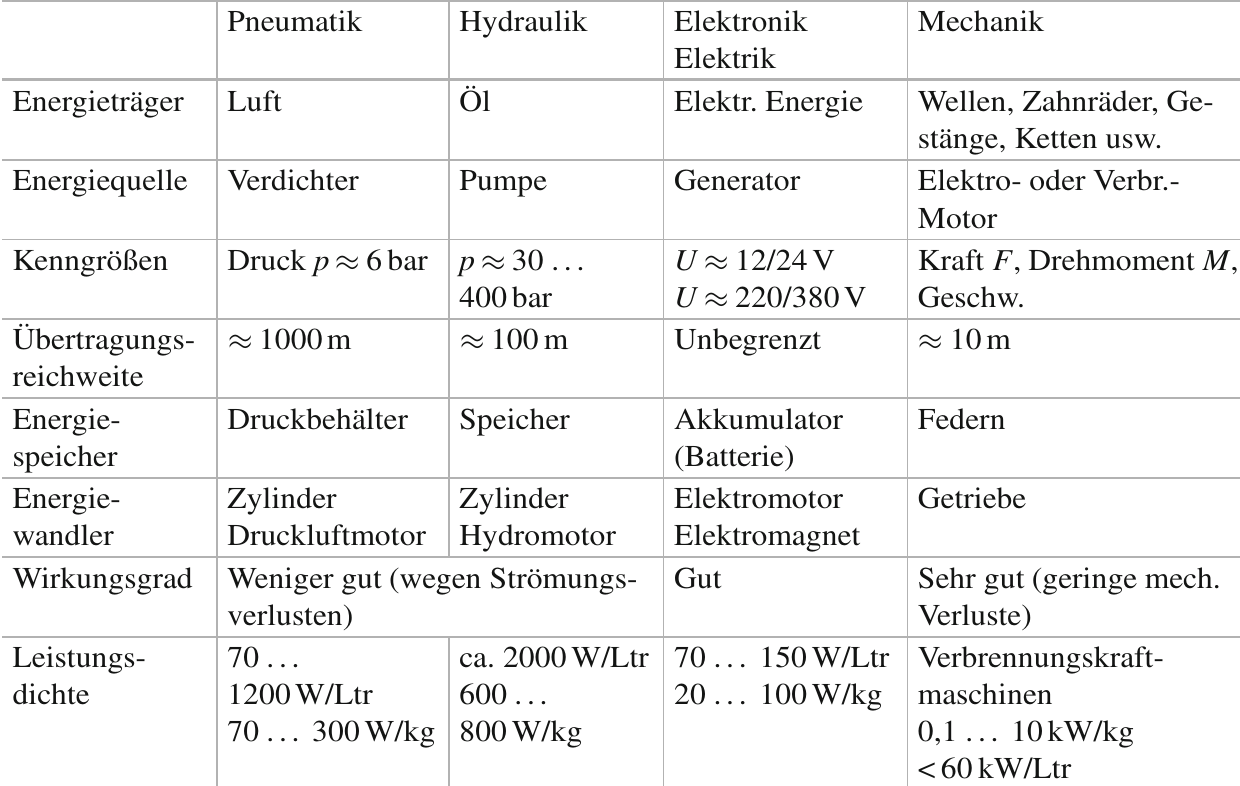
\includegraphics[width=\linewidth]{./ch01.basics/pics/compareDrives}  
  
  \vspace*{-1.0\baselineskip}{\tiny\color{red}Aus Sicherheitsgr\"unden wird bei der Pneumatik kein h\"oherer Druck 
  verwendet.}
  %%= = = = = = = = = = = = = = = = = = = = = = = = = = = = = = = = = = = = = =

\end{frame}
%= = = = = = = = = = = = = = = = = = = = = = = = = = = = = = = = = = = = = = =

% \part{Kombi}
% \section{Hydraulische und Pneumatische Bauteile}
\subsection{Grundlagen}
%= = = = = = = = = = = = = = = = = = = = = = = = = = = = = = = = = = = = = = =
%= = = = = = = = = = = = = = = = = = = = = = = = = = = = = = = = = = = = = = =
% \iffalse
\begin{frame}
  \frametitle{Eigenschaften der Fluide}
%  \framesubtitle{H\"oren}
  %%= = = = = = = = = = = = = = = = = = = = = = = = = = = = = = = = = = = = = =
  Anforderungen
  \begin{itemize}
    \item Temperatur-\adSTField{Viskosit\"ats}verhalten,
    \item gute Schmier- und \adSTField{Verschlei\ss{}schutz}eigenschaften 
      (h\"aufig Mischreibungsbedingungen bei kleinen Gleitgeschwindigkeiten),
    \item gute \adSTField{Korrosionsschutz}eigenschaften und gute 
      Lack- und Dichtungsvertr\"aglichkeit (Gummi, Kunststoffe, Buntmetalle),
    \item Alterungsbest\"andigkeit (\adSTField{Oxidation}, Harzbildung durch Polymerisation)
  \end{itemize}
  
   \ifteacher%%
   \else%%
    %  \vspace*{-0.7\baselineskip}\hspace{\stretch{1}}\rotatebox[origin=lB]{180}{%%
     \vspace*{-1.0\baselineskip}\hspace{\stretch{1}}\rotatebox[origin=lB]{180}{%%
     \resizebox{0.9\linewidth}{!}{\parbox[t]{3.95\linewidth}{%%
    %  \tiny
   %   \vspace*{-0.7\baselineskip}\hspace*{0.95\linewidth-1cm}\makebox[0pt][l]{\rotatebox[origin=c]{180}{\resizebox{1cm}{!}{%
     Viskosit\"ats, Verschlei\ss{}schutz, Korrosionsschutz, Oxidation
     }}}
   \fi%%
  
  %%= = = = = = = = = = = = = = = = = = = = = = = = = = = = = = = = = = = = = =

\end{frame}
%= = = = = = = = = = = = = = = = = = = = = = = = = = = = = = = = = = = = = = =

% \part{Kombi}
% \section{Hydraulische und Pneumatische Bauteile}
% \subsection{Grundlagen}
%= = = = = = = = = = = = = = = = = = = = = = = = = = = = = = = = = = = = = = =
%= = = = = = = = = = = = = = = = = = = = = = = = = = = = = = = = = = = = = = =
% \iffalse
\begin{frame}
  \frametitle{Eigenschaften der Fluide: Dichte $\rho$}
%  \framesubtitle{H\"oren}
  %%= = = = = = = = = = = = = = = = = = = = = = = = = = = = = = = = = = = = = =
  \vspace{-2\baselineskip}
  \[
    \rho = \frac{m}{V}\quad \left[\unit{\frac{kg}{m^3}}\right]
  \]  
  Im technischen Gebrauch liegt die Dichte $\rho$ der verwendeten Fluiden 
  (Hydraulik\"ol oder Druckfl\"ussigkeit) bei 
  % \teacherfalse
  \adSTFieldm{\unitfrac[900]{kg}{m^3}}.

  Bei steigender Temperatur wird das Volumen bei gleichbleibender Masse 
  gr\"o\ss{}er, die Dichte verringert sich daher mit dem Volums\"anderungskoeffizient
  $\alpha$:
  \[-\frac{\Delta\rho}{\rho}\approx\frac{\Delta V}{V}=\alpha \cdot \Delta \theta;
  \quad \begin{array}[c]{@{}l@{}}
        \rho_\theta =\rho_{15^\circ{}\mathrm{C}}+\adSTFieldm{\Delta \rho} \approx 
        \rho_{15^\circ{}\mathrm{C}} \cdot (1-\adSTFieldm{\alpha\cdot\Delta \theta}) \\
        V_\theta =V_{15^\circ{}\mathrm{C}}+\adSTFieldm{\Delta V} = 
        V_{15^\circ{}\mathrm{C}} \cdot (1+\adSTFieldm{\alpha\cdot\Delta \theta}) \\
        \end{array}\]

  % \adRule{6}{9}      
  \parbox[t]{0.45\linewidth}{%
  \begin{tabular}[t]{@{}rl@{}}
    $V$ & \adSTField{Volumen}\\
    $\Delta V$ & Volums\adSTField{\"anderung}\\
    $\rho_{15^\circ{}\mathrm{C}}$ & \adSTField{Dichte} bei $\unit[15]{^\circ{}C}$\\
    $\rho_\theta$ & Dichte bei \adSTField{Temperatur} $\theta$
  \end{tabular}
  }\hspace{\stretch{1}}\parbox[t]{0.53\linewidth}{%
  F\"ur die meisten Hydraulik\"ole ist der Volumenkorrekturfaktor 
  $\alpha \approx \unitfrac[0.70\cdot10^{-3}]{1}{K}$
  }

   \ifteacher%%
   \else%%
    %  \vspace*{-0.7\baselineskip}\hspace{\stretch{1}}\rotatebox[origin=lB]{180}{%%
     \vspace*{-1.0\baselineskip}\hspace{\stretch{1}}\rotatebox[origin=lB]{180}{%%
     \resizebox{0.9\linewidth}{!}{\parbox[t]{3.95\linewidth}{%%
    %  \tiny
   %   \vspace*{-0.7\baselineskip}\hspace*{0.95\linewidth-1cm}\makebox[0pt][l]{\rotatebox[origin=c]{180}{\resizebox{1cm}{!}{%
     $\Delta \rho$, $\alpha\cdot\Delta \theta$, $\Delta V$, $\alpha\cdot\Delta \theta$
     $\unitfrac[900]{kg}{m^3}$, Volumen, \"anderung, Dichte, Temperatur, 
     }}}
   \fi%%
  
  %%= = = = = = = = = = = = = = = = = = = = = = = = = = = = = = = = = = = = = =

\end{frame}
%= = = = = = = = = = = = = = = = = = = = = = = = = = = = = = = = = = = = = = =

% \part{Kombi}
% \section{Hydraulische und Pneumatische Bauteile}
% \subsection{Grundlagen}
%= = = = = = = = = = = = = = = = = = = = = = = = = = = = = = = = = = = = = = =
%= = = = = = = = = = = = = = = = = = = = = = = = = = = = = = = = = = = = = = =
% \iffalse
\begin{frame}
  \frametitle{Eigenschaften der Fluide: Dichte $\rho$}
%  \framesubtitle{H\"oren}
  %%= = = = = = = = = = = = = = = = = = = = = = = = = = = = = = = = = = = = = =
  \begin{block}{Beispiel: Dichte\"anderung bei Temperaturerh\"ohung}
    Bsp.: $\unit[2.5]{kg}$ eines Hydraulik\"oles mit einer Dichte von 
    $\unitfrac[900]{kg}{m^3}$ bei $\unit[15]{^\circ\,C}$ wird auf 
    $\unit[95]{^\circ\,C}$ erwärmt.
  Bestimmen Sie das Volumen.

  \end{block}


   \ifteacher%%
   \else%%
    %  \vspace*{-0.7\baselineskip}\hspace{\stretch{1}}\rotatebox[origin=lB]{180}{%%
     \vspace*{-1.0\baselineskip}\hspace{\stretch{1}}\rotatebox[origin=lB]{180}{%%
     \resizebox{0.9\linewidth}{!}{\parbox[t]{3.95\linewidth}{%%
    %  \tiny
   %   \vspace*{-0.7\baselineskip}\hspace*{0.95\linewidth-1cm}\makebox[0pt][l]{\rotatebox[origin=c]{180}{\resizebox{1cm}{!}{%
     \ %%
     }}}
   \fi%%
  
  %%= = = = = = = = = = = = = = = = = = = = = = = = = = = = = = = = = = = = = =

\end{frame}
%= = = = = = = = = = = = = = = = = = = = = = = = = = = = = = = = = = = = = = =

% \part{Kombi}
% \section{Hydraulische und Pneumatische Bauteile}
% \subsection{Grundlagen}
%= = = = = = = = = = = = = = = = = = = = = = = = = = = = = = = = = = = = = = =
%= = = = = = = = = = = = = = = = = = = = = = = = = = = = = = = = = = = = = = =
% \iffalse
\begin{frame}
  \frametitle{Eigenschaften der Fluide: Kompressibilit\"at}
%  \framesubtitle{H\"oren}
  %%= = = = = = = = = = = = = = = = = = = = = = = = = = = = = = = = = = = = = =
  Bei zunehmendem Druck komprimiert sich das \"Ol, der Zusammenhang 
  f\"ur das Dichte-Druck-Verhalten ist im linearisiertem Modell:

  \[
    \frac{\Delta\rho}{\rho}\approx-\frac{\Delta V}{V}=\beta \cdot \Delta p;
    \quad \begin{array}[c]{@{}l@{}}
      \rho_p =\rho_{p_0}+\adSTFieldm{\Delta \rho} \approx 
      \rho_{p_0} \cdot (1+\adSTFieldm{\beta\cdot\Delta p})     \\
      V_p =V_{p_0}+\adSTFieldm{\Delta V} = 
      V_{p_0} \cdot (1-\adSTFieldm{\beta\cdot\Delta p}) \\
      \end{array}
  \]


  \begin{tabular}[t]{@{}rl@{}}
    $V$ & \adSTField{Volumen}\\
    $\Delta V$ & Volums\adSTField{\"anderung}\\
    $\rho_{p_0}$ & \adSTField{Dichte} bei Normaldruck $p_0$\\
    $\rho_p$ & Dichte bei veränderten \adSTField{Druck} $p$\\
    $\beta$ &  \adSTField{Kompressibilit\"at}/Pressziffer in $\left[\unitfrac[]{1}{bar}\right]$\\
    $K=\nicefrac[]{1}{\beta}$ & Kompressionsmodul/\adSTField{Elastizit\"atsmodul} in $\left[\unit[]{bar}\right]$ 
  \end{tabular}

   \ifteacher%%
   \else%%
    %  \vspace*{-0.7\baselineskip}\hspace{\stretch{1}}\rotatebox[origin=lB]{180}{%%
     \vspace*{-1.0\baselineskip}\hspace{\stretch{1}}\rotatebox[origin=lB]{180}{%%
     \resizebox{0.9\linewidth}{!}{\parbox[t]{3.95\linewidth}{%%
    %  \tiny
   %   \vspace*{-0.7\baselineskip}\hspace*{0.95\linewidth-1cm}\makebox[0pt][l]{\rotatebox[origin=c]{180}{\resizebox{1cm}{!}{%
     $\Delta \rho$, $\beta\cdot\Delta p$, $\Delta V$, $\beta\cdot\Delta p$,\\
     Volumen, \"anderung, Dichte, Druck, Kompressibilit\"at, Elastizit\"atsmodul
     }}}
   \fi%%
  
  %%= = = = = = = = = = = = = = = = = = = = = = = = = = = = = = = = = = = = = =

\end{frame}
%= = = = = = = = = = = = = = = = = = = = = = = = = = = = = = = = = = = = = = =

% \part{Kombi}
% \section{Hydraulische und Pneumatische Bauteile}
% \subsection{Grundlagen}
%= = = = = = = = = = = = = = = = = = = = = = = = = = = = = = = = = = = = = = =
%= = = = = = = = = = = = = = = = = = = = = = = = = = = = = = = = = = = = = = =
% \iffalse
\begin{frame}
  \frametitle{Eigenschaften der Fluide: Kompressibilit\"at}
%  \framesubtitle{H\"oren}
  %%= = = = = = = = = = = = = = = = = = = = = = = = = = = = = = = = = = = = = =

  \begin{block}{Beispiel: Dichte\"anderung unter Druck}
    Bsp.: $\unit[2.5]{kg}$ eines Hydraulik\"oles mit einer Dichte von 
    $\unitfrac[900]{kg}{m^3}$ bei einem Druck von $p_0=\unit[1]{bar}$ 
    wird unter einen Druck von $p=\unit[150]{bar}$ komprimiert.
  Bestimmen Sie das Volumen.

  \begin{tabular}[]{@{}rll}
    \toprule
    & Kompressionsmodul $K$ & Kompressibilität $\beta$\\
    \"Olsorte & in $10^4$ bar & in $10^{-4}$ \unitfrac[]{1}{bar} \\
    \midrule
    Mineral\"ol &1.4 & 0.7\\
    HFC, HFD-Hydraulik\"ol & 3 & \nicefrac{1}{3} $\approx$ 0.33\\
    \bottomrule
  \end{tabular}

  Aus \emph{Hydraulik und Pneumatik, 2017}
  \end{block}


   \ifteacher%%
   \else%%
    %  \vspace*{-0.7\baselineskip}\hspace{\stretch{1}}\rotatebox[origin=lB]{180}{%%
     \vspace*{-1.0\baselineskip}\hspace{\stretch{1}}\rotatebox[origin=lB]{180}{%%
     \resizebox{0.9\linewidth}{!}{\parbox[t]{3.95\linewidth}{%%
    %  \tiny
   %   \vspace*{-0.7\baselineskip}\hspace*{0.95\linewidth-1cm}\makebox[0pt][l]{\rotatebox[origin=c]{180}{\resizebox{1cm}{!}{%
     Volumen, \"anderung, Dichte, Temperatur, $\unitfrac[900]{kg}{m^3}$
     }}}
   \fi%%
  
  %%= = = = = = = = = = = = = = = = = = = = = = = = = = = = = = = = = = = = = =

\end{frame}
%= = = = = = = = = = = = = = = = = = = = = = = = = = = = = = = = = = = = = = =

% \part{Kombi}
% \section{Hydraulische und Pneumatische Bauteile}
% \subsection{Grundlagen}
%= = = = = = = = = = = = = = = = = = = = = = = = = = = = = = = = = = = = = = =
%= = = = = = = = = = = = = = = = = = = = = = = = = = = = = = = = = = = = = = =
% \iffalse
\begin{frame}
  \frametitle{Eigenschaften der Fluide: Viskosit\"at, \emph{Rheologie}}
%  \framesubtitle{H\"oren}
  %%= = = = = = = = = = = = = = = = = = = = = = = = = = = = = = = = = = = = = =
  
  Die Viskosit\"at ist ein Ma\ss{} f\"ur den \adSTField{Flie\ss{}widerstand}, die Z\"ahigkeit
  auf Grund der inneren \adSTField{Reibung} (dick- und d\"unnfl\"ussg).

  \parbox[c]{0.51\linewidth}{
    In einem linearem \adSTField{Modell} (nach \textsc{Isaac NEWTON} werden zwei parallele 
    Platten mit einer \adSTField{Fl\"ache} $A$,
    die sich mit einer \adSTField{Relativgeschwindigkeit} $v$ zueinander bewegen und 
    in einem \adSTField{Abstand} $d=\Delta y$ sind, betrachtet.
  }\hspace{\stretch{1}}\parbox[c]{0.48\linewidth}{
      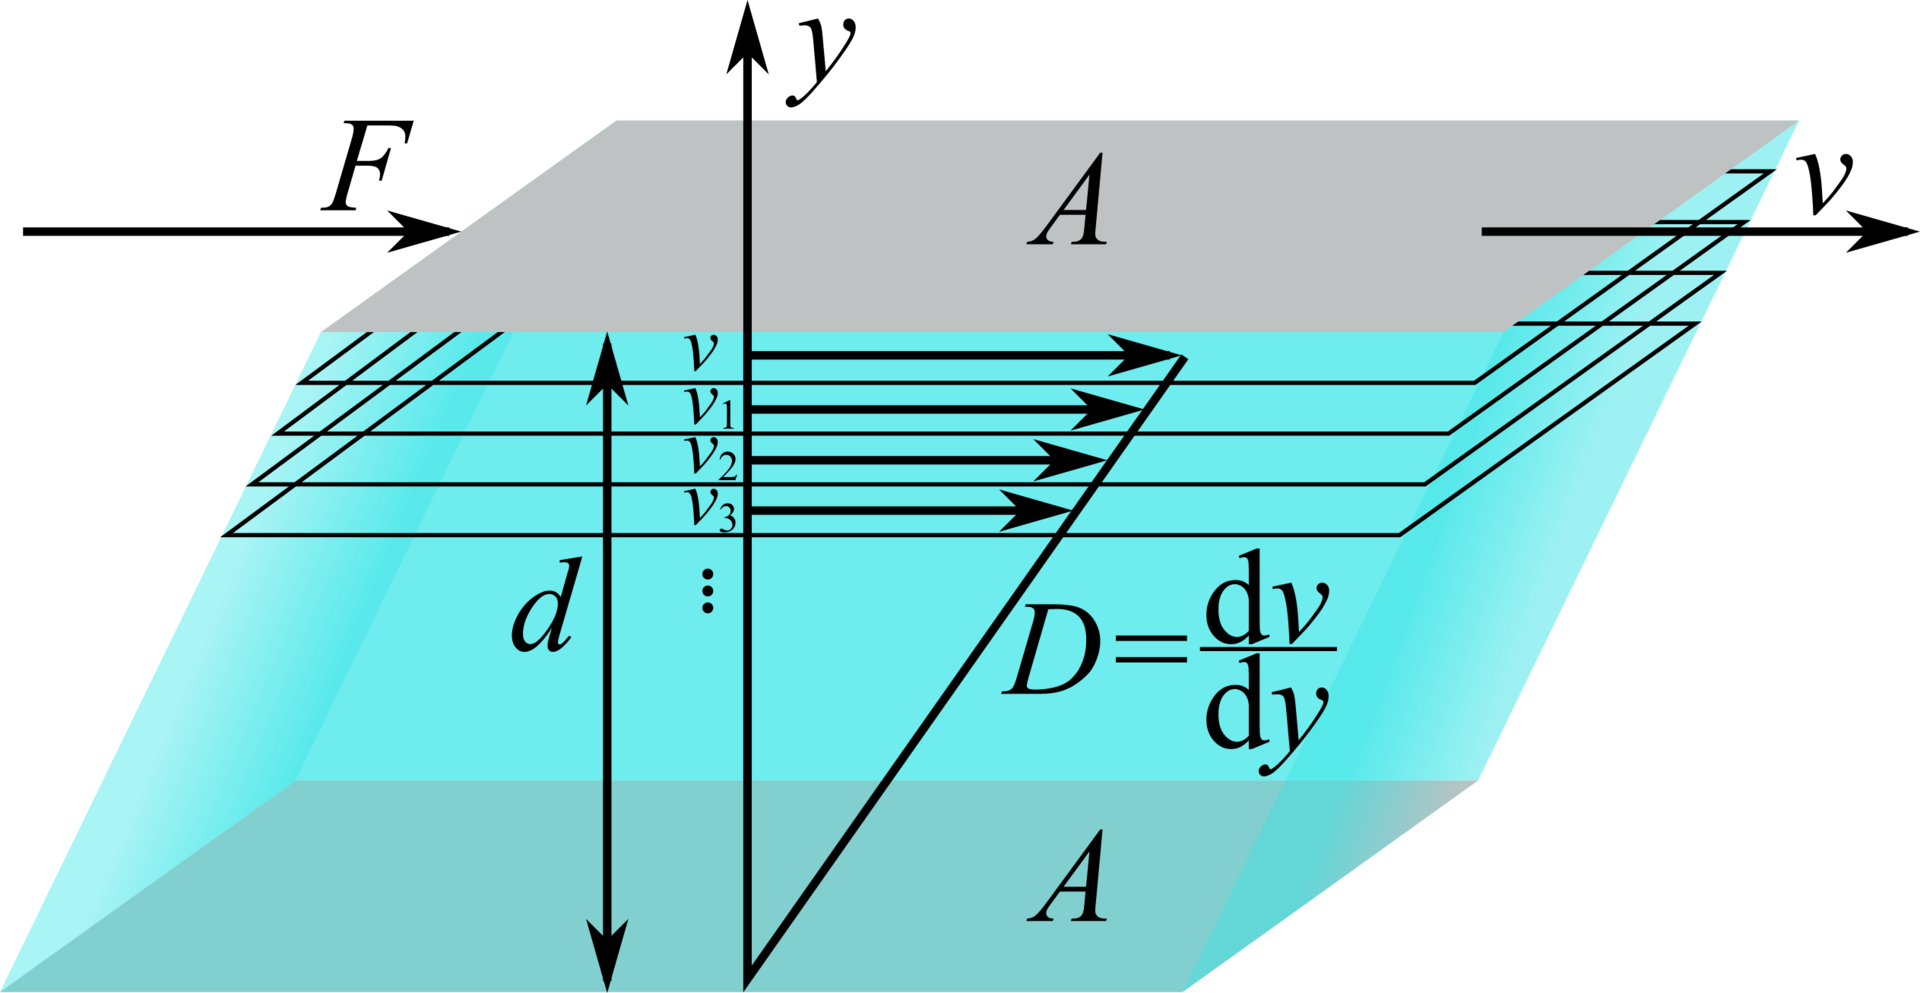
\includegraphics[width=\linewidth]{./ch01.basics/pics/Definition_Viskositaet}
  } 

  \ifteacher%%
  \else%%
   %  \vspace*{-0.7\baselineskip}\hspace{\stretch{1}}\rotatebox[origin=lB]{180}{%%
    \vspace*{-0.0\baselineskip}\hspace{\stretch{1}}\rotatebox[origin=lB]{180}{%%
    \resizebox{0.9\linewidth}{!}{\parbox[t]{3.95\linewidth}{%%
   %  \tiny
  %   \vspace*{-0.7\baselineskip}\hspace*{0.95\linewidth-1cm}\makebox[0pt][l]{\rotatebox[origin=c]{180}{\resizebox{1cm}{!}{%
  Flie\ss{}widerstand, Reibung, Modell, Fl\"ache, Relativgeschwindigkeit, Abstand
    }}}
  \fi%%
  
  %%= = = = = = = = = = = = = = = = = = = = = = = = = = = = = = = = = = = = = =

\end{frame}
%= = = = = = = = = = = = = = = = = = = = = = = = = = = = = = = = = = = = = = =

% \part{Kombi}
% \section{Hydraulische und Pneumatische Bauteile}
% \subsection{Grundlagen}
%= = = = = = = = = = = = = = = = = = = = = = = = = = = = = = = = = = = = = = =
%= = = = = = = = = = = = = = = = = = = = = = = = = = = = = = = = = = = = = = =
% \iffalse
\begin{frame}
  \frametitle{Eigenschaften der Fluide: Viskosit\"at, \emph{Rheologie}}
%  \framesubtitle{H\"oren}
  %%= = = = = = = = = = = = = = = = = = = = = = = = = = = = = = = = = = = = = =
  
  \begin{tabular}[t]{@{}lll@{}}
    je gr\"o\ss{}er die Fl\"ache & desto \adSTField{gr\"o\ss{}er} die Kraft & $F\sim A$\\
    je gr\"o\ss{}er die Geschwindigkeit & desto \adSTField{gr\"o\ss{}er} die Kraft & $F\sim \Delta v\ (\diff{v})$\\
    je gr\"o\ss{}er der Abstand der Platten & desto \adSTField{kleiner} die Kraft & $F \sim \nicefrac[]{1}{\Delta y}\ (\nicefrac[]{1}{\diff{y}})$
  \end{tabular}
  

  Mit dem materialabh\"angigen Proportionalit\"atfaktor $\eta$ 
  (absolute oder dynamische Viskosit\"at) erh\"alt man (im einfachen linearen Modell):
  \parbox[c]{0.49\linewidth}{
    \[
      F = \eta \cdot A \cdot \frac{\Delta v}{\Delta y}= \eta \cdot A \cdot \frac{\diff{v}}{\diff{y}}
    \] 
  }\hspace{\stretch{1}}\parbox[c]{0.49\linewidth}{
    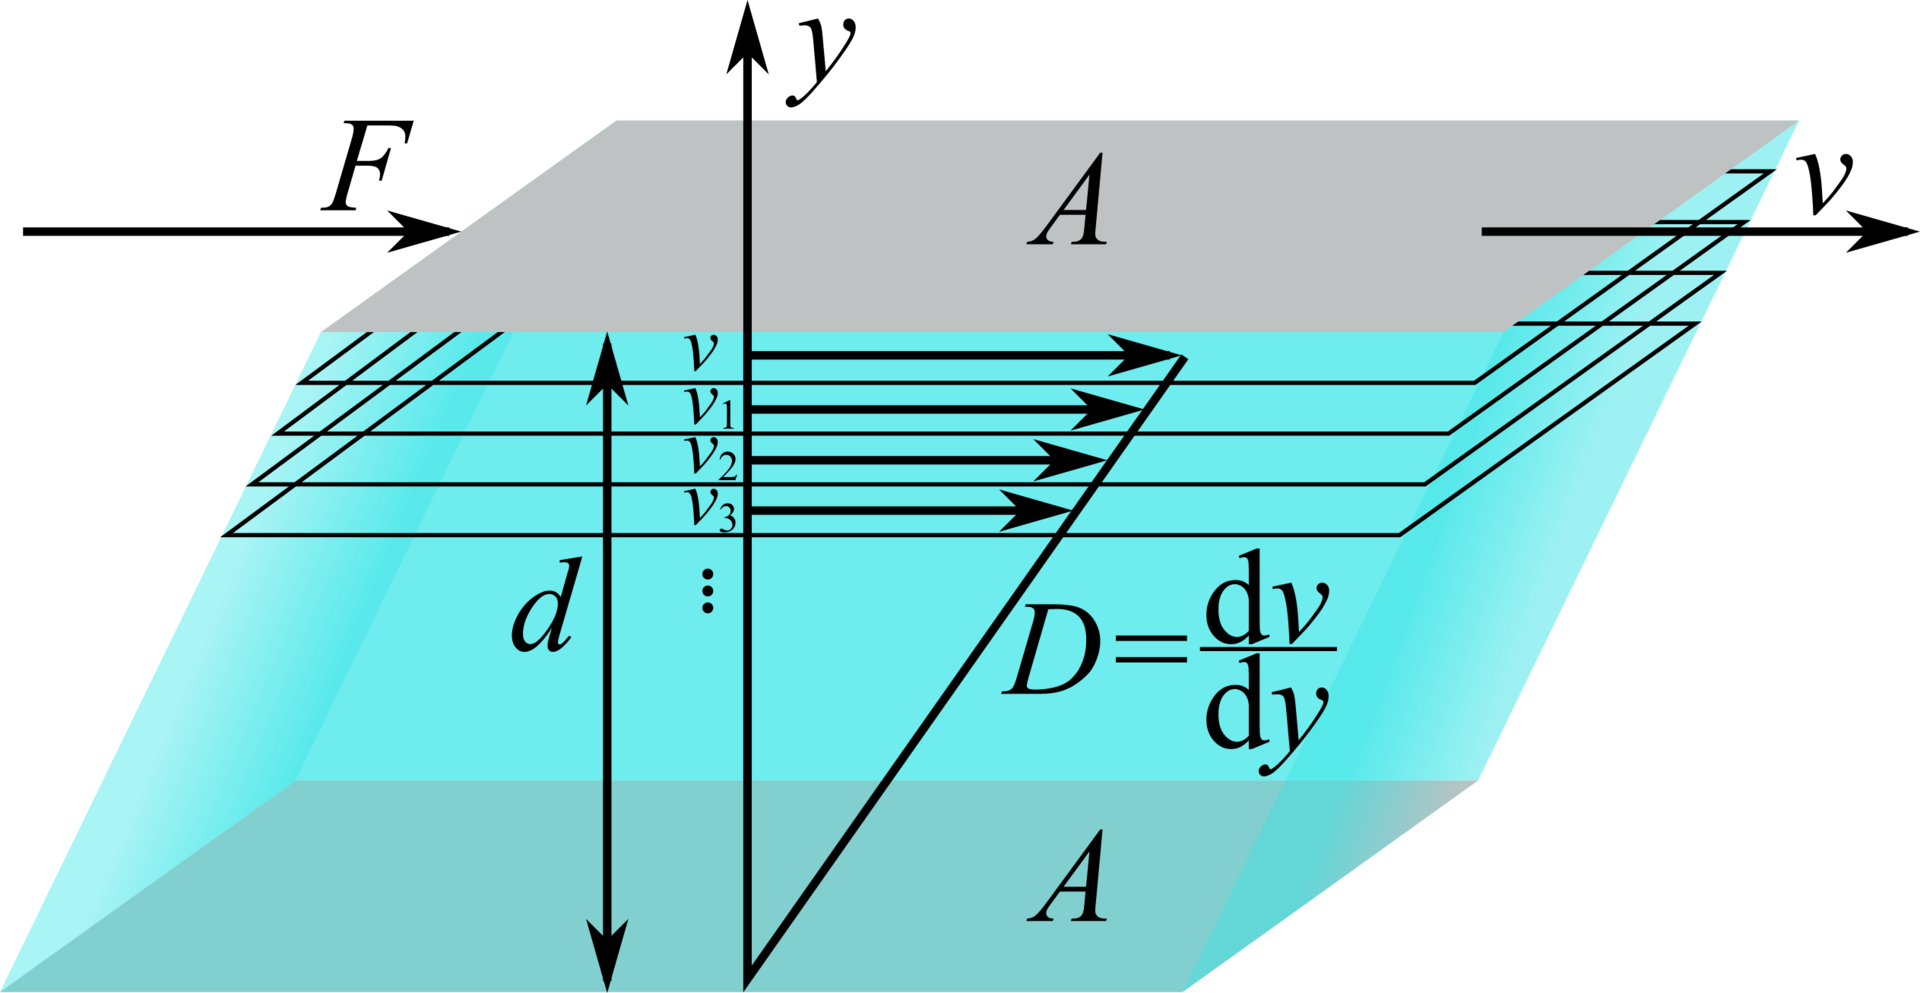
\includegraphics[width=\linewidth]{./ch01.basics/pics/Definition_Viskositaet}
  }

  \ifteacher%%
  \else%%
   %  \vspace*{-0.7\baselineskip}\hspace{\stretch{1}}\rotatebox[origin=lB]{180}{%%
    \vspace*{-1.0\baselineskip}\hspace{\stretch{1}}\rotatebox[origin=lB]{180}{%%
    \resizebox{0.9\linewidth}{!}{\parbox[t]{3.95\linewidth}{%%
   %  \tiny
  %   \vspace*{-0.7\baselineskip}\hspace*{0.95\linewidth-1cm}\makebox[0pt][l]{\rotatebox[origin=c]{180}{\resizebox{1cm}{!}{%
  gr\"o\ss{}er, gr\"o\ss{}er, kleiner
    }}}
  \fi%%

  % \begin{block}{Beispiel: Dichte\"anderung unter Druck}
  %   Bsp.: $\unit[2.5]{kg}$ eines Hydraulik\"oles mit einer Dichte von 
  %   $\unitfrac[900]{kg}{m^3}$ bei einem Druck von $p_0=\unit[1]{bar}$ 
  %   wird unter einen Druck von $p=\unit[150]{bar}$ komprimiert.
  % Bestimmen Sie das Volumen.

  %%= = = = = = = = = = = = = = = = = = = = = = = = = = = = = = = = = = = = = =

\end{frame}
%= = = = = = = = = = = = = = = = = = = = = = = = = = = = = = = = = = = = = = =

% \part{Kombi}
% \section{Hydraulische und Pneumatische Bauteile}
% \subsection{Grundlagen}
%= = = = = = = = = = = = = = = = = = = = = = = = = = = = = = = = = = = = = = =
%= = = = = = = = = = = = = = = = = = = = = = = = = = = = = = = = = = = = = = =
% \iffalse
\begin{frame}
  \frametitle{Eigenschaften der Fluide: Viskosit\"at, \emph{Rheologie}}
%  \framesubtitle{H\"oren}
  %%= = = = = = = = = = = = = = = = = = = = = = = = = = = = = = = = = = = = = =
  Die Viskosit\"at \"andert sich mit:
  \begin{itemize}
    \item \adSTField{Temperatur}
    \item \adSTField{Druck}
    \item \adSTField{Geschwindigkeit}
    \item Alterung
  \end{itemize}
  
  Durch Zugabe von Additiven wird versucht, die Eigenschaften des Hydraulik\"oles
  f\"ur den Betrieb zu verbessern, und Alterungsvorg\"ange zu verlangsamen.

  \ifteacher%%
  \else%%
   %  \vspace*{-0.7\baselineskip}\hspace{\stretch{1}}\rotatebox[origin=lB]{180}{%%
    \vspace*{-1.0\baselineskip}\hspace{\stretch{1}}\rotatebox[origin=lB]{180}{%%
    \resizebox{0.9\linewidth}{!}{\parbox[t]{3.95\linewidth}{%%
   %  \tiny
  %   \vspace*{-0.7\baselineskip}\hspace*{0.95\linewidth-1cm}\makebox[0pt][l]{\rotatebox[origin=c]{180}{\resizebox{1cm}{!}{%
  Temperatur, Druck, Geschwindigkeit
    }}}
  \fi%%

  % \begin{block}{Beispiel: Dichte\"anderung unter Druck}
  %   Bsp.: $\unit[2.5]{kg}$ eines Hydraulik\"oles mit einer Dichte von 
  %   $\unitfrac[900]{kg}{m^3}$ bei einem Druck von $p_0=\unit[1]{bar}$ 
  %   wird unter einen Druck von $p=\unit[150]{bar}$ komprimiert.
  % Bestimmen Sie das Volumen.

  %%= = = = = = = = = = = = = = = = = = = = = = = = = = = = = = = = = = = = = =

\end{frame}
%= = = = = = = = = = = = = = = = = = = = = = = = = = = = = = = = = = = = = = =



% \part{Kombi}
% \section{Hydraulische und Pneumatische Bauteile}
% \subsection{Grundlagen}
%= = = = = = = = = = = = = = = = = = = = = = = = = = = = = = = = = = = = = = =
%= = = = = = = = = = = = = = = = = = = = = = = = = = = = = = = = = = = = = = =
% \iffalse
\begin{frame}
  \frametitle{Kennbuchstaben }
%  \framesubtitle{H\"oren}
  %%= = = = = = = = = = = = = = = = = = = = = = = = = = = = = = = = = = = = = =
  \begin{tabular}[t]{@{}ll@{\quad}ll@{}}
    \toprule
    AN  & Normalschmieröle,                    & Jx  & elektrische Isolieröle,             \\
    Bx  & Schmieröl BA, BB oder                &     & JA oder JB,                         \\
        & BC (z. B.: bitumenhaltig),           & Kx  & Kältemaschinenöle,                  \\
    C   & Umlaufschmieröle,                    & L   & Härte- und Vergüteöle,              \\
    CG  & Gleitbahnöle,                        & Q   & Wärmeträgeröle,                     \\
    D   & Druckluftöle,                        & R   & Korrosionsschutzöle,                \\
    F   & Luftfilteröle,                       & S   & Kühlschmierstoffe,                  \\
    FS  & Formen-Trennöle,                     & TD  & Schmier- und Regleröle,             \\
    H   & Hydrauliköle,                        & V   & Luftverdichteröle,                  \\
    HF  & schwer entflammbare Hydraulik\"ole,  & W   & Walzöle,                            \\
    HE  & biologisch abbaubare Hydraulik\"ole, & Zx  & Dampfzylinderöle.                   \\ 
    HV  & Hydrauliköle mit verbessertem        &     & ZS, ZA, ZB oder ZD.\\
        & Viskositäts-Temperatur-Verhalten, \\
    \bottomrule
  \end{tabular}

  \ifteacher%%
  \else%%
   %  \vspace*{-0.7\baselineskip}\hspace{\stretch{1}}\rotatebox[origin=lB]{180}{%%
    \vspace*{-1.0\baselineskip}\hspace{\stretch{1}}\rotatebox[origin=lB]{180}{%%
    \resizebox{0.9\linewidth}{!}{\parbox[t]{3.95\linewidth}{%%
   %  \tiny
  %   \vspace*{-0.7\baselineskip}\hspace*{0.95\linewidth-1cm}\makebox[0pt][l]{\rotatebox[origin=c]{180}{\resizebox{1cm}{!}{%
  Temperatur, Druck, Geschwindigkeit
    }}}
  \fi%%

  % \begin{block}{Beispiel: Dichte\"anderung unter Druck}
  %   Bsp.: $\unit[2.5]{kg}$ eines Hydraulik\"oles mit einer Dichte von 
  %   $\unitfrac[900]{kg}{m^3}$ bei einem Druck von $p_0=\unit[1]{bar}$ 
  %   wird unter einen Druck von $p=\unit[150]{bar}$ komprimiert.
  % Bestimmen Sie das Volumen.

  %%= = = = = = = = = = = = = = = = = = = = = = = = = = = = = = = = = = = = = =

\end{frame}
%= = = = = = = = = = = = = = = = = = = = = = = = = = = = = = = = = = = = = = =


% \part{Kombi}
% \section{Hydraulische und Pneumatische Bauteile}
% \subsection{Grundlagen}
%= = = = = = = = = = = = = = = = = = = = = = = = = = = = = = = = = = = = = = =
%= = = = = = = = = = = = = = = = = = = = = = = = = = = = = = = = = = = = = = =
% \iffalse
\begin{frame}
  \frametitle{Umwelteinfl\"ussse}
%  \framesubtitle{H\"oren}
  %%= = = = = = = = = = = = = = = = = = = = = = = = = = = = = = = = = = = = = =
  Von etwa \adSTField{1.3 Millionen} Tonnen pro Jahr abgesetzte Mineral\"ole werden
  rund \adSTField{0.75 Millionen} Tonnen dem Recycling zur\"uckgef\"uhrt. Der Rest 
  verbleibt in der Natur als \adSTField{Verlustschmierung} oder Havarien, ein 
  Teil landet durch Verbrennung als CO$_2$ in der Atmosp\"are.
  (Zahlen f\"ur Deutschland).

  Umweltvertr\"agliche Hydraulikfl\"usssigkeiten sind biologisch 
  \adSTField{schnell} abbaubar und nicht \adSTField{toxisch}
  (harmlos bis zu einer Konzentration von \unitfrac[10...100]{ml}{l}).
  Als Basis f\"ur derartige \"Ole dienen sowohl 
  \begin{description}
    \item[nat\"urliche Rohstoffe] (Sonnenblumen, Raps, \dots )
    \item[mineralische \"Ole] 
    \item[syntetische Stoffe] Mischung aus nat\"urlichen und mineralischen.
  \end{description}
  Die Kosten belaufen sich f\"ur vergleichbare Qualit\"aten auf etwa das 
  Doppelte.
    
  % Einige Projekte 
  % besch\"aftigen sich mit dieser Problematik, sei es ernsthaft
  %  oder zur Kosmetik.


  \ifteacher%%
  \else%%
   %  \vspace*{-0.7\baselineskip}\hspace{\stretch{1}}\rotatebox[origin=lB]{180}{%%
    \vspace*{-0.10\baselineskip}\hspace{\stretch{1}}\rotatebox[origin=lB]{180}{%%
    \resizebox{0.9\linewidth}{!}{\parbox[t]{3.95\linewidth}{%%
   %  \tiny
  %   \vspace*{-0.7\baselineskip}\hspace*{0.95\linewidth-1cm}\makebox[0pt][l]{\rotatebox[origin=c]{180}{\resizebox{1cm}{!}{%
  1.3 Millionen, 0.75 Millionen, Verlustschmierung, schnell, toxisch
    }}}
  \fi%%

  %%= = = = = = = = = = = = = = = = = = = = = = = = = = = = = = = = = = = = = =

\end{frame}
%= = = = = = = = = = = = = = = = = = = = = = = = = = = = = = = = = = = = = = =

% \part{Kombi}
% \section{Hydraulische und Pneumatische Bauteile}
% \subsection{Grundlagen}
%= = = = = = = = = = = = = = = = = = = = = = = = = = = = = = = = = = = = = = =
%= = = = = = = = = = = = = = = = = = = = = = = = = = = = = = = = = = = = = = =
% \iffalse
\begin{frame}
  \frametitle{Eigenschaften der Druckluft}
%  \framesubtitle{H\"oren}
  %%= = = = = = = = = = = = = = = = = = = = = = = = = = = = = = = = = = = = = =
  Luft besteht im Wesentlichen aus \unit[79]{\%$_\mathrm{Vol}$} 
  \adSTField{Stickstoff} N$_2$
  $\approx$ \unit[21]{\%$_\mathrm{Vol}$}  \adSTField{Sauerstoff} O$_2$ und 
  weniger als  \unit[1]{\%$_\mathrm{Vol}$}  \adSTField{Edelgase}. 
  Die Druckluft muss frei von Partikeln sein und eine möglichst geringe
  \adSTField{Luftfeuchtigkeit} besitzen.  
  
  \ifteacher%%
  \else%%
   %  \vspace*{-0.7\baselineskip}\hspace{\stretch{1}}\rotatebox[origin=lB]{180}{%%
    \vspace*{-0.10\baselineskip}\hspace{\stretch{1}}\rotatebox[origin=lB]{180}{%%
    \resizebox{0.9\linewidth}{!}{\parbox[t]{3.95\linewidth}{%%
   %  \tiny
  %   \vspace*{-0.7\baselineskip}\hspace*{0.95\linewidth-1cm}\makebox[0pt][l]{\rotatebox[origin=c]{180}{\resizebox{1cm}{!}{%
  Stickstoff, Sauerstoff, Edelgase, Luftfeuchtigkeit
    }}}
  \fi%%

  %%= = = = = = = = = = = = = = = = = = = = = = = = = = = = = = = = = = = = = =

\end{frame}
%= = = = = = = = = = = = = = = = = = = = = = = = = = = = = = = = = = = = = = =


% \part{Kombi}
% \section{Hydraulische und Pneumatische Bauteile}
% \subsection{Grundlagen}
%= = = = = = = = = = = = = = = = = = = = = = = = = = = = = = = = = = = = = = =
%= = = = = = = = = = = = = = = = = = = = = = = = = = = = = = = = = = = = = = =
% \iffalse
\begin{frame}
  \frametitle{Zustands\"anderung}
%  \framesubtitle{H\"oren}
  %%= = = = = = = = = = = = = = = = = = = = = = = = = = = = = = = = = = = = = =
  \parbox[t]{0.4\linewidth}{%
    Die Dichte $\rho$ der Luft ist nicht konstant. F\"ur das ideale 
    Gas gilt:
    \[
      p \cdot V = m \cdot R \cdot T = N \cdot k_\mathrm{B} \cdot T
    \]
  }\hspace{\stretch{1}}\parbox[t]{0.58\linewidth}{%
  \vspace*{-0.7\baselineskip}\begin{tabular}[t]{@{}l@{\,\dots\,}l@{}}
    \toprule
    $m$ & \adSTField{Stoffmenge} in Mol\\
    $R$ & \adSTField{Gaskonst.} ($\unitfrac[8.314]{J}{mol K}$) \\
    $N$ & \adSTField{Molek\"ulanzahl}\\
    $k_\mathrm{B}$ & \adSTField{Boltzmannkonst.} $\unitfrac[1.38 \cdot 10^{-23}]{J}{K}$\\
    \bottomrule
  \end{tabular}
  }
    
  Abh\"angig von der Art und Weise 
  der \adSTField{Zustands\"anderung} gilt n\"aherungsweise (an das ideale Gasgesetz 
  angelehnt):
  \[
    p \cdot V^n = \mathrm{const.}
  \]
  
  \parbox[t]{0.54\linewidth}{%
    % Für 
    \begin{description}
      \item[isotherme] Zustands\"anderungen $n=1$
      \item[adiabatische] Zustands\"anderungen $n=\kappa$, $\kappa=\frac{c_p}{c_v} \approx 1.4$  
    \end{description}
  }\hspace{\stretch{1}}\parbox[t]{0.45\linewidth}{%
  \vspace*{-0.7\baselineskip}\begin{tabular}[t]{@{}l@{\,}l@{}}
    \toprule
    $c_p$\,\dots & spez. W\"armekapazit\"at\\
          & bei $p=$konst. $\approx \unitfrac[1]{kJ}{kg K}$\\
    $c_V$\,\dots & spez. W\"armekapazit\"at\\
          & bei $V=$konst. $\approx \unitfrac[0.72]{kJ}{kg K}$\\
    \bottomrule
  \end{tabular}
  }

  \ifteacher%%
  \else%%
   %  \vspace*{-0.7\baselineskip}\hspace{\stretch{1}}\rotatebox[origin=lB]{180}{%%
    \vspace*{-0.10\baselineskip}\hspace{\stretch{1}}\rotatebox[origin=lB]{180}{%%
    \resizebox{0.9\linewidth}{!}{\parbox[t]{3.95\linewidth}{%%
   %  \tiny
  %   \vspace*{-0.7\baselineskip}\hspace*{0.95\linewidth-1cm}\makebox[0pt][l]{\rotatebox[origin=c]{180}{\resizebox{1cm}{!}{%
  Stoffmenge, Rydberkonstante, Molek\"ulanzahl, Boltzmannkonstante, Zustands\"anderung
    }}}
  \fi%%

  %%= = = = = = = = = = = = = = = = = = = = = = = = = = = = = = = = = = = = = =

\end{frame}
%= = = = = = = = = = = = = = = = = = = = = = = = = = = = = = = = = = = = = = =

% \part{Kombi}
% \section{Hydraulische und Pneumatische Bauteile}
% \subsection{Grundlagen}
%= = = = = = = = = = = = = = = = = = = = = = = = = = = = = = = = = = = = = = =
%= = = = = = = = = = = = = = = = = = = = = = = = = = = = = = = = = = = = = = =
% \iffalse
\begin{frame}
  \frametitle{Molvolumen, Dichte}
%  \framesubtitle{H\"oren}
  %%= = = = = = = = = = = = = = = = = = = = = = = = = = = = = = = = = = = = = =
  Aus dem idealem Gasgesetz erh\"alt man unter \adSTFieldm{Normbedingungen}
  ($p=\unit[101300]{pa}, T=\unit[273]{K}$) das molare \adSTFieldm{Volumen}:
  \[
    V = 1\cdot \frac{R\cdot T}{p} \approx \unit[0.0224]{m^3}= \unit[22.4]{l}%\unit[1.27]{kg}
  \]

  Mit der Molmasse von $m_{\mathrm{O}_2} = \unit[32]{g}$ und $m_{\mathrm{N}_2} = \unit[28]{g}$
  ergibt sich f\"ur die \adSTFieldm{Masse} von \unit[1]{mol} Luft
  \[
    m_\mathrm{Luft} = \nicefrac{1}{5} \cdot m_{\mathrm{O}_2}
                      + \nicefrac{4}{5} \cdot m_{\mathrm{N}_2}
                    \approx \unit[28.8]{g}
  \]
  
  Damit erh\"alt man die \adSTFieldm{Dichte}
  \[
    \rho_\mathrm{Luft} = \frac{m_\mathrm{Luft}}{V} = \frac{28.8}{0.0224}\approx \unitfrac[1.29]{kg}{m^3}
  \]

  \ifteacher%%
  \else%%
   %  \vspace*{-0.7\baselineskip}\hspace{\stretch{1}}\rotatebox[origin=lB]{180}{%%
    \vspace*{-0.10\baselineskip}\hspace{\stretch{1}}\rotatebox[origin=lB]{180}{%%
    \resizebox{0.9\linewidth}{!}{\parbox[t]{3.95\linewidth}{%%
   %  \tiny
  %   \vspace*{-0.7\baselineskip}\hspace*{0.95\linewidth-1cm}\makebox[0pt][l]{\rotatebox[origin=c]{180}{\resizebox{1cm}{!}{%
    Normbedingungen, Volumen, Masse, Dichte
    }}}
  \fi%%

  % \begin{block}{Beispiel: Dichte\"anderung unter Druck}
  %   Bsp.: $\unit[2.5]{kg}$ eines Hydraulik\"oles mit einer Dichte von 
  %   $\unitfrac[900]{kg}{m^3}$ bei einem Druck von $p_0=\unit[1]{bar}$ 
  %   wird unter einen Druck von $p=\unit[150]{bar}$ komprimiert.
  % Bestimmen Sie das Volumen.

  %%= = = = = = = = = = = = = = = = = = = = = = = = = = = = = = = = = = = = = =

\end{frame}
%= = = = = = = = = = = = = = = = = = = = = = = = = = = = = = = = = = = = = = =


% \part{Kombi}
% \section{Hydraulische und Pneumatische Bauteile}
% \subsection{Grundlagen}
%= = = = = = = = = = = = = = = = = = = = = = = = = = = = = = = = = = = = = = =
%= = = = = = = = = = = = = = = = = = = = = = = = = = = = = = = = = = = = = = =
% \iffalse
\begin{frame}
  \frametitle{\"Ubersicht Zustands\"anderungen}
%  \framesubtitle{H\"oren}
  %%= = = = = = = = = = = = = = = = = = = = = = = = = = = = = = = = = = = = = =
  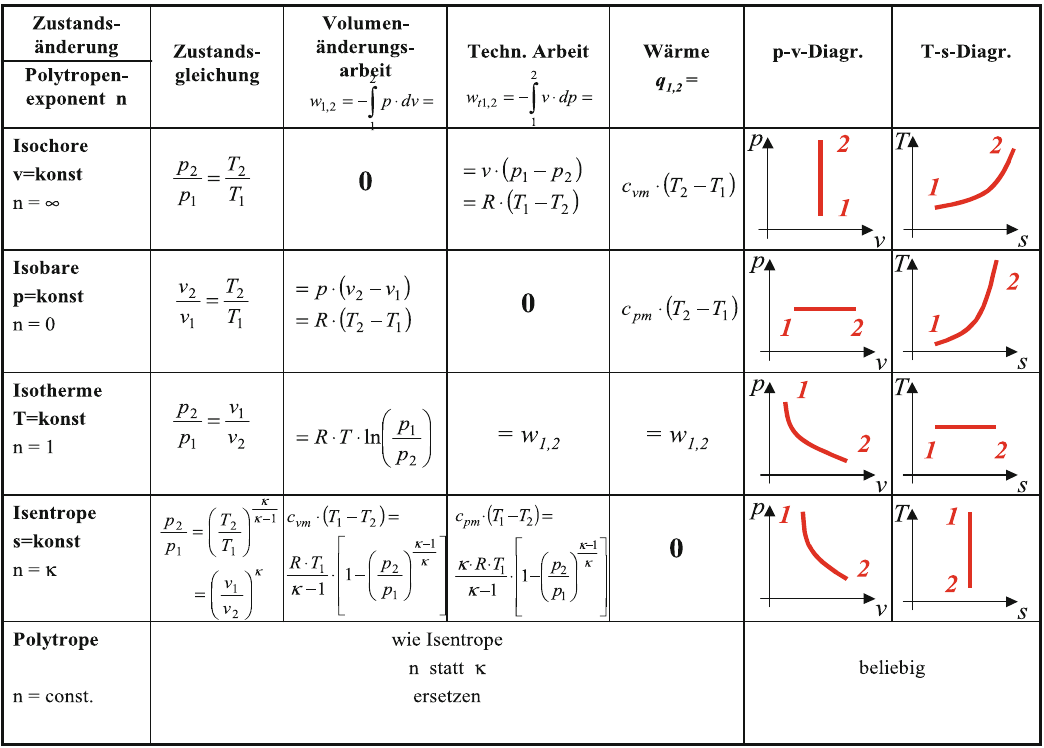
\includegraphics[width=0.90\linewidth]{./ch01.basics/pics/zustandsaenderung}
  \ifteacher%%
  \else%%
   %  \vspace*{-0.7\baselineskip}\hspace{\stretch{1}}\rotatebox[origin=lB]{180}{%%
    \vspace*{-0.10\baselineskip}\hspace{\stretch{1}}\rotatebox[origin=lB]{180}{%%
    \resizebox{0.9\linewidth}{!}{\parbox[t]{3.95\linewidth}{%%
   %  \tiny
  %   \vspace*{-0.7\baselineskip}\hspace*{0.95\linewidth-1cm}\makebox[0pt][l]{\rotatebox[origin=c]{180}{\resizebox{1cm}{!}{%
      \ %
    }}}
  \fi%%

  % \begin{block}{Beispiel: Dichte\"anderung unter Druck}
  %   Bsp.: $\unit[2.5]{kg}$ eines Hydraulik\"oles mit einer Dichte von 
  %   $\unitfrac[900]{kg}{m^3}$ bei einem Druck von $p_0=\unit[1]{bar}$ 
  %   wird unter einen Druck von $p=\unit[150]{bar}$ komprimiert.
  % Bestimmen Sie das Volumen.

  %%= = = = = = = = = = = = = = = = = = = = = = = = = = = = = = = = = = = = = =

\end{frame}
%= = = = = = = = = = = = = = = = = = = = = = = = = = = = = = = = = = = = = = =

% \part{Kombi}
% \section{Hydraulische und Pneumatische Bauteile}
% \subsection{Grundlagen}
%= = = = = = = = = = = = = = = = = = = = = = = = = = = = = = = = = = = = = = =
%= = = = = = = = = = = = = = = = = = = = = = = = = = = = = = = = = = = = = = =
% \iffalse
\begin{frame}
  \frametitle{Druck $p$}
%  \framesubtitle{H\"oren}
  %%= = = = = = = = = = = = = = = = = = = = = = = = = = = = = = = = = = = = = =
  \begin{block}{Druck $p$}
    \parbox[c]{0.43\linewidth}{%%
    Der statische Druck ist definiert als}
    \parbox[c]{0.15\linewidth}{%% 
    \[ p=\frac{F}{A}\] }
    \parbox[c]{0.4\linewidth}{%%
    mit der Einheit \unit[1]{Pascal} = \unit[1]{pa}.}
    
    In der Technik wird 
    die Einheit \unit[1]{Bar}=\unit[10$^\text{5}$]{pa} verwendet, was 
    den hydrostatischen Druck von \unit[10]{m} Wassers\"aule entspricht.
  \end{block}
  \begin{block}{Druckenergie $\Delta\,W_p$}
    Wird unter Druckeinwirkung die Fl\"ache $A$ um den Weg 
    $\Delta\,s$ verschoben, so ergibt sich
    mit der Volumen\"anderungsarbeit bei gleichbleibendem Druck $p$ 
    mit dem verschobenen Volumen $\Delta\,V$
    \[
      \Delta\,W_p = F \cdot \Delta\,s = p \cdot A \cdot \Delta\,s = p \cdot \Delta\,V
    \]
  \end{block}
  

  \ifteacher%%
  \else%%
   %  \vspace*{-0.7\baselineskip}\hspace{\stretch{1}}\rotatebox[origin=lB]{180}{%%
    \vspace*{-0.50\baselineskip}\hspace{\stretch{1}}\rotatebox[origin=lB]{180}{%%
    \resizebox{0.9\linewidth}{!}{\parbox[t]{3.95\linewidth}{%%
    \ \\
    \ .
   %  \tiny
  %   \vspace*{-0.7\baselineskip}\hspace*{0.95\linewidth-1cm}\makebox[0pt][l]{\rotatebox[origin=c]{180}{\resizebox{1cm}{!}{%
    \ %
    }}}
  \fi%%

  % \begin{block}{Beispiel: Dichte\"anderung unter Druck}
  %   Bsp.: $\unit[2.5]{kg}$ eines Hydraulik\"oles mit einer Dichte von 
  %   $\unitfrac[900]{kg}{m^3}$ bei einem Druck von $p_0=\unit[1]{bar}$ 
  %   wird unter einen Druck von $p=\unit[150]{bar}$ komprimiert.
  % Bestimmen Sie das Volumen.

  %%= = = = = = = = = = = = = = = = = = = = = = = = = = = = = = = = = = = = = =

\end{frame}
%= = = = = = = = = = = = = = = = = = = = = = = = = = = = = = = = = = = = = = =

% \part{Kombi}
% \section{Hydraulische und Pneumatische Bauteile}
% \subsection{Grundlagen}
%= = = = = = = = = = = = = = = = = = = = = = = = = = = = = = = = = = = = = = =
%= = = = = = = = = = = = = = = = = = = = = = = = = = = = = = = = = = = = = = =
% \iffalse
\begin{frame}
  \frametitle{Druckenergie}
%  \framesubtitle{H\"oren}
  %%= = = = = = = = = = = = = = = = = = = = = = = = = = = = = = = = = = = = = =
  \begin{block}{Bsp. Druckspeicher}
    % Es soll ein Druckspeicher mit einem Volumen $V=$\unit[10]{l}
    % unter einen Druck von $p=$\unit[4]{bar} gef\"ullt werden.

    Ein Druckspeicher mit Volumen $V$=\unit[10]{l}
    wird mit einem Druck von $p$=\unit[4]{bar} gef\"ullt.

    \begin{description}
      \item[i)] Berechnen Sie die dazu notwendige Arbeit $W_\mathrm{in}$,
        % um den Druckspeicher zu f\"ullen.
      \item[ii)] Berechnen Sie die verwertbare Energie, nachdem die Luft 
        im Speicher wieder Umgebungstemperatur erreicht hat.
    \end{description}
  \end{block}
  \begin{block}{Bsp. Druckspeicher: Modellierung}
    \textsc{i}) Das Komprimieren findet im Normalfall so schnell statt, dass keine 
    Energie mit der Aussenwelt ausgetauscht werden kann $\Longrightarrow$ 
    adiabatische Zustands\"anderung.

    \textsc{ii}) Danach k\"uhlt die komprimierte Luft wieder auf Umgebungstemperatur 
    ab $\Longrightarrow$ isochore Zustands\"anderung.

    \textsc{iii}) Am Arbeitsger\"at entspannt sich die Luft langsam, sodass sie 
    die Temperatur der Umgebungstemperatur aufrechterh\"alt 
    $\Longrightarrow$ isotherme Zustands\"anderung.

    % \[
    %   \Delta\,W_p = F \cdot \Delta\,s = p \cdot A \cdot \Delta\,s = p \cdot \Delta\,V
    % \]
  \end{block}
  

  \ifteacher%%
  \else%%
   %  \vspace*{-0.7\baselineskip}\hspace{\stretch{1}}\rotatebox[origin=lB]{180}{%%
    \vspace*{-0.10\baselineskip}\hspace{\stretch{1}}\rotatebox[origin=lB]{180}{%%
    \resizebox{0.9\linewidth}{!}{\parbox[t]{3.95\linewidth}{%%
   %  \tiny
  %   \vspace*{-0.7\baselineskip}\hspace*{0.95\linewidth-1cm}\makebox[0pt][l]{\rotatebox[origin=c]{180}{\resizebox{1cm}{!}{%
    \ %
    }}}
  \fi%%
  %%= = = = = = = = = = = = = = = = = = = = = = = = = = = = = = = = = = = = = =

\end{frame}
%= = = = = = = = = = = = = = = = = = = = = = = = = = = = = = = = = = = = = = =

% \part{Kombi}
% \section{Hydraulische und Pneumatische Bauteile}
% \subsection{Grundlagen}
%= = = = = = = = = = = = = = = = = = = = = = = = = = = = = = = = = = = = = = =
%= = = = = = = = = = = = = = = = = = = = = = = = = = = = = = = = = = = = = = =
% \iffalse
\begin{frame}
  \frametitle{Druckenergie}
%  \framesubtitle{H\"oren}
  %%= = = = = = = = = = = = = = = = = = = = = = = = = = = = = = = = = = = = = =
  \begin{block}{Bsp. Druckspeicher, $V$=\unit[10]{l}, $p$=\unit[4]{bar}, i)}
    Adiabatische Zustands\"anderung: $p \cdot V^\kappa$=const.
  \end{block}
  \begin{block}{Bsp. Druckspeicher: Modellierung}
    % \[
    %   \Delta\,W_p = F \cdot \Delta\,s = p \cdot A \cdot \Delta\,s = p \cdot \Delta\,V
    % \]
  \end{block}
  

  \ifteacher%%
  \else%%
   %  \vspace*{-0.7\baselineskip}\hspace{\stretch{1}}\rotatebox[origin=lB]{180}{%%
    \vspace*{-0.10\baselineskip}\hspace{\stretch{1}}\rotatebox[origin=lB]{180}{%%
    \resizebox{0.9\linewidth}{!}{\parbox[t]{3.95\linewidth}{%%
   %  \tiny
  %   \vspace*{-0.7\baselineskip}\hspace*{0.95\linewidth-1cm}\makebox[0pt][l]{\rotatebox[origin=c]{180}{\resizebox{1cm}{!}{%
    \ %
    }}}
  \fi%%
  %%= = = = = = = = = = = = = = = = = = = = = = = = = = = = = = = = = = = = = =

\end{frame}
%= = = = = = = = = = = = = = = = = = = = = = = = = = = = = = = = = = = = = = =

% \part{Kombi}
% \section{Intro}
% \subsection*{Intro}
% %= = = = = = = = = = = = = = = = = = = = = = = = = = = = = = = = = = = = = = =
% %= = = = = = = = = = = = = = = = = = = = = = = = = = = = = = = = = = = = = = =
% % \iffalse
% \begin{frame}
%   \frametitle{Intro}
% %  \framesubtitle{H\"oren}
%   %%= = = = = = = = = = = = = = = = = = = = = = = = = = = = = = = = = = = = = =
%   Todo
%   what ist
%   %%= = = = = = = = = = = = = = = = = = = = = = = = = = = = = = = = = = = = = =
%
% \end{frame}
% %= = = = = = = = = = = = = = = = = = = = = = = = = = = = = = = = = = = = = = =

% \part{Kombi}
\section{Intro}
% \subsection*{Intro}
% \input{ch04.matrices/chapter/matrices.intro.tex}

% \include{chapter/statistics.intro}
% \include{chapter/ch01/stat.ch01.01.basics}
% \include{chapter/ch01/stat.ch01.02.parameter.tex}
% \include{chapter/ch02/stat.ch02.01.stat.inference.intro}
% \include{ch04.matrices/matrices.main.tex}
% \include{chapter/ch01/prob.ch01.permutations.II}
% \include{chapter/ch01/prob.ch01.combinations}
% \include{chapter/ch01/prob.ch01.conclusion}
%
\end{document}


